\documentclass[a4paper]{article}
\usepackage{vntex}
\usepackage{a4wide,amssymb,epsfig,latexsym,multicol,array,hhline,fancyhdr}
\usepackage{fancybox}
\usepackage{amsmath}
\usepackage{lastpage}
\usepackage[lined,boxed,commentsnumbered]{algorithm2e}
\usepackage{enumerate}
\usepackage{color}
\usepackage{graphicx}							
\usepackage{array}
\usepackage{tabularx, caption}
\usepackage{multirow}
\usepackage{listings}
\usepackage{xcolor}
\lstset { %
    language=C++,
    backgroundcolor=\color{black!5}, % set backgroundcolor
    basicstyle=\footnotesize,% basic font setting
}
\usepackage{multicol}
\usepackage{arydshln}
\usepackage{rotating}
\usepackage{graphics}
\usepackage{geometry}
\usepackage{setspace}
\usepackage{indentfirst}
\usepackage{epsfig}
\usepackage{tikz}
\usetikzlibrary{arrows,snakes,backgrounds}
\usepackage{hyperref}
\hypersetup{urlcolor=blue,linkcolor=black,citecolor=black,colorlinks=true} 
\setlength{\headheight}{40pt}
\pagestyle{fancy}
\fancyhead{} 
\fancyhead[L]{
 \begin{tabular}{rl}
    \begin{picture}(25,15)(0,0)
    \put(0,-8){
\includegraphics[width=8mm, height=8mm]{hcmut.png}}
   \end{picture}&
	\begin{tabular}{l}
		\textbf{\bf \ttfamily Trường Đại Học Bách Khoa Tp.Hồ Chí Minh}\\
		\textbf{\bf \ttfamily Khoa Khoa Học và Kỹ Thuật Máy Tính}
	\end{tabular} 	
 \end{tabular}
}
\fancyhead[R]{
	\begin{tabular}{l}
		\tiny \bf \\
		\tiny \bf 
	\end{tabular}  }
\fancyfoot{} 
\fancyfoot[L]{\scriptsize \ttfamily Assignment 2 - Kĩ thuật lập trình}
\fancyfoot[R]{\scriptsize \ttfamily Trang {\thepage}/\pageref{LastPage}}
\renewcommand{\headrulewidth}{0.3pt}
\renewcommand{\footrulewidth}{0.3pt--}


%%%
\setcounter{secnumdepth}{4}
\setcounter{tocdepth}{3}
\makeatletter
\newcounter {subsubsubsection}[subsubsection]
\renewcommand\thesubsubsubsection{\thesubsubsection .\@alph\c@subsubsubsection}
\newcommand\subsubsubsection{\@startsection{subsubsubsection}{4}{\z@}%
                                     {-3.25ex\@plus -1ex \@minus -.2ex}%
                                     {1.5ex \@plus .2ex}%
                                     {\normalfont\normalsize\bfseries}}
\newcommand*\l@subsubsubsection{\@dottedtocline{3}{10.0em}{4.1em}}
\newcommand*{\subsubsubsectionmark}[1]{}
\makeatother


\begin{document}
\thispagestyle{empty}
\thisfancypage{
\setlength{\fboxsep}{10pt}
\fbox}{} 
\begin{titlepage}
\begin{center}
ĐẠI HỌC QUỐC GIA THÀNH PHỐ HỒ CHÍ MINH \\
TRƯỜNG ĐẠI HỌC BÁCH KHOA \\
KHOA KHOA HỌC - KỸ THUẬT MÁY TÍNH 
\end{center}

\vspace{1cm}

\begin{figure}[h!]
\begin{center}

\includegraphics[width=3cm]{hcmut.png}
\end{center}
\end{figure}

\vspace{1cm}


\begin{center}
\begin{tabular}{l}
\multicolumn{1}{l}{\textbf{{\Large Kĩ thuật lập trình}}}\\
~~\\
\hline
\\
\multicolumn{1}{l}{\textbf{{\Large Assignment 2:  Thiết kế phần  mềm quản lý thư viện}}}\\
\\
\hline
\end{tabular}
\end{center}
\vspace{1cm}
\begin{center}
\vspace{1cm}
\end{center}
\begin{center}
\begin{tabular}{rlc}
Sinh Viên: &Vũ Hoàng Văn  \hspace{1cm}     & 1614063 \\
&Nguyễn Văn Tường	&1614028\\
&Huỳnh Phúc Nghị	&1612233\\
&Lương Tuấn Kiệt & 1611695\\

\end{tabular}
\end{center}
\vspace{3.2cm}
\begin{center}
{\footnotesize TP. HỒ CHÍ MINH, THÁNG 6/2017}
\end{center}
\end{titlepage}
\newpage
\thispagestyle{empty}
\tableofcontents

%Danh sách bảng
\newpage
\thispagestyle{empty}
\listoftables

%Danh sách hình
\newpage
\thispagestyle{empty}
\listoffigures

\newpage

\section{Tổ chức nhóm}
	\begin{table}[!h]
		\begin{center}
			\begin{tabular}{|c|c|c|c|c|}
				\hline 
				Sinh viên & MSSV & Thành phần & Tỉ lệ điểm & Ghi chú \\ 
				\hline 
		   	 	Huỳnh Phúc Nghị & 1612233 & Sơ đồ, giải thuật, tester & 25\%&   \\ 
			    \hline 
			    Lương Tuấn Kiệt & 1611695 & Thiết kế mã nguồn, cơ sở dữ liệu & 25\%&  \\ 
				\hline 
				Nguyễn Văn Tường & 1614028 & Thiết kế giao diện & 25\% &\\ 
				\hline 
				Vũ Hoàng Văn & 1614063 & Thiết kế tính năng & 25\% &\\ 
				\hline 
			\end{tabular} 
			\caption{Bảng tổ chức nhóm}
		\end{center}
	\end{table}
	Trao đổi giữa các thành viên trong nhóm:	
	\begin{itemize}
	\item Trao đổi ý tưởng: Facebook
	\item Trao đổi mã nguồn: Git + Github
	\item Công cụ hỗ trợ code: Qt Creator
	\item Công cụ biên dịch: Qt 5.9, qmake
	\item Công cụ soạn thảo báo cáo: TexMaker + Texlive
	\item Công cụ vẽ lưu đồ giải thuật và các cấu trúc: \url{http://draw.io}

	\end{itemize}
\newpage
\section{Khảo sát và Phân tích yêu cầu của phần mềm}
Yêu cầu đề bài: Thiết kế một phần mềm hỗ trợ các hoạt động diễn ra hằng ngày ở một thư viện.
\begin{itemize}
\item Yêu cầu chính: Thiết kế một phần mềm hỗ trợ quản lý cho một thư viện
\item Thiết kế giải thuật phù hợp với các yêu cầu tùy theo người sử dụng
\item Thiết kế giao diện tương tác với từng vai trò người sử dụng
\item Với độc giả (Reader): Thiết kế tính năng tìm tài liệu, gửi yêu cầu mượn tài liệu, xem tài liệu đã mượn,...
\item Với thủ thư (Librarian): Thiết kế tính năng quản lý tài liệu, quản lý yêu cầu mượn tài liệu,...
\item Với quản lý (Admin): Thiết kế tính năng quản lý, chỉnh sửa, thêm bớt tài khoản, nhận khiếu nại, góp ý từ người sử dụng
\end{itemize}
Các tính năng cần có của phần mềm:
\begin{itemize}
\item Có giao diện giúp người dùng đăng nhập / đăng xuất dễ dàng cùng tài khoản của họ
\item Có khả năng hiển thị danh sách sách sẵn có trong thư viện, thông tin về sách, khả năng chỉnh sửa cũng như thêm/bớt sách vào thư viện
\item Có khả năng tương tác/quản lý các yêu cầu mượn sách, trả sách, mất sách từ người dùng
\item Có khả năng quản lý, chỉnh sửa, thêm bớt các tài khoản, vai trò của các tài khoản trong hệ thống
\item Thiết kế code minh bạch, tổ chức rõ ràng, giao diện thân thiện
\end{itemize}


\section{Thiết kế phần mềm}
\subsection{Thiết kế các cấu trúc dữ liệu dùng để phát triển phần mềm thư viện}
Nêu sơ đồ thiết kế bằng hình ảnh và diễn giải. Đối với các lớp hay cấu trúc, có thể trịch code đặt tại đây, nhưng cần ngắn gọn.
\begin{itemize}
	\item Dữ liệu tương tác: lớp User.\\
	\begin{figure}[h!]
	\begin{center}
		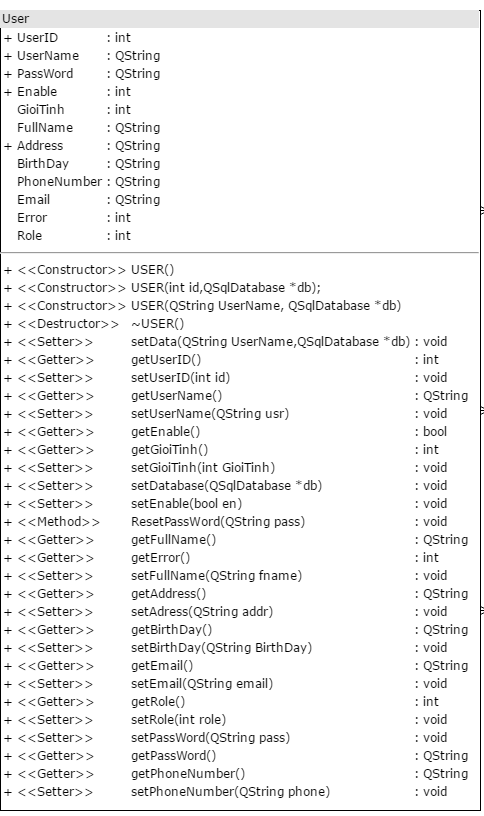
\includegraphics[scale=.8]{Diagram_User.png}
		\caption{Class User}
	\end{center}
	\end{figure}
	\newpage \newpage 
	\item Các lớp cửa sổ tương ứng: Cửa sổ chính, cửa sổ đăng nhập, cửa sổ ứng với từng vai trò,...
	\item Phương thức lưu trữ / truy xuất dữ liệu: ngôn ngữ cơ sở dữ liệu SQLITE tích hợp trong Qt
\end{itemize}
Các lệnh tương tác với cơ sở dữ liệu trong ngôn ngữ Sql:\\
\begin{itemize}
\item SELECT: chọn từ cơ sở dữ liệu các đối tượng thỏa mãn một điều kiện cụ thể
\item INSERT: thêm vào cơ sở dữ liệu một đối tượng mới 
\item DELETE: xóa các đối tượng từ cơ sở dữ liệu thỏa theo điều kiện cụ thể 
\item UPDATE: chỉnh sửa các đối tượng thuộc cơ sở dữ liệu thỏa theo điều kiện cụ thể
\end{itemize}
\subsection{Thiết kế các khối chức năng và hệ thống con}
\begin{figure}[h!]
	\begin{center}
		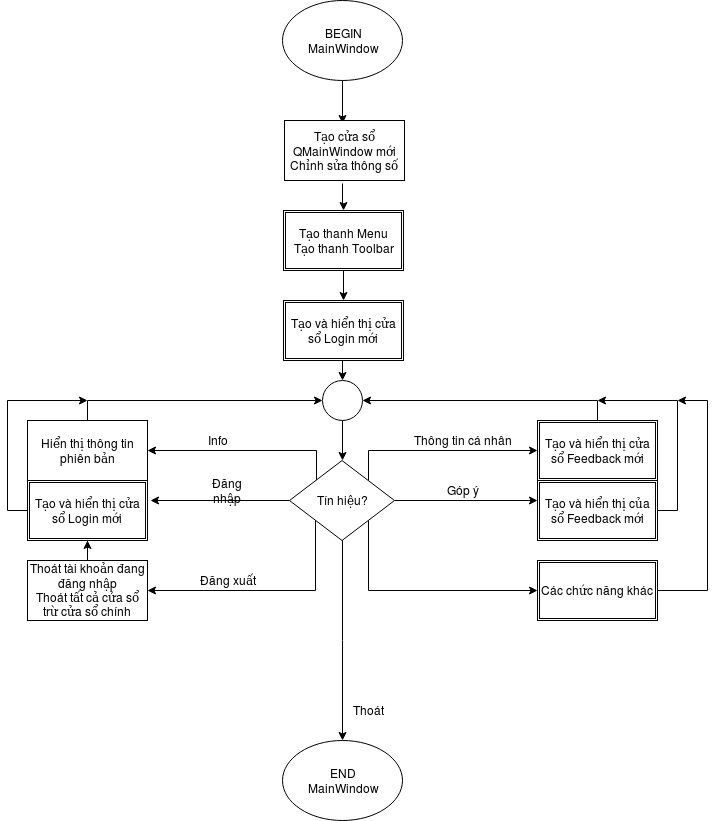
\includegraphics[scale=.5]{mainDiagram.png}
		\caption{Sơ đồ hoạt động chính của LIBPRO}
	\end{center}
	\end{figure}
	\newpage \newpage 
\begin{figure}[h!]
	\begin{center}
		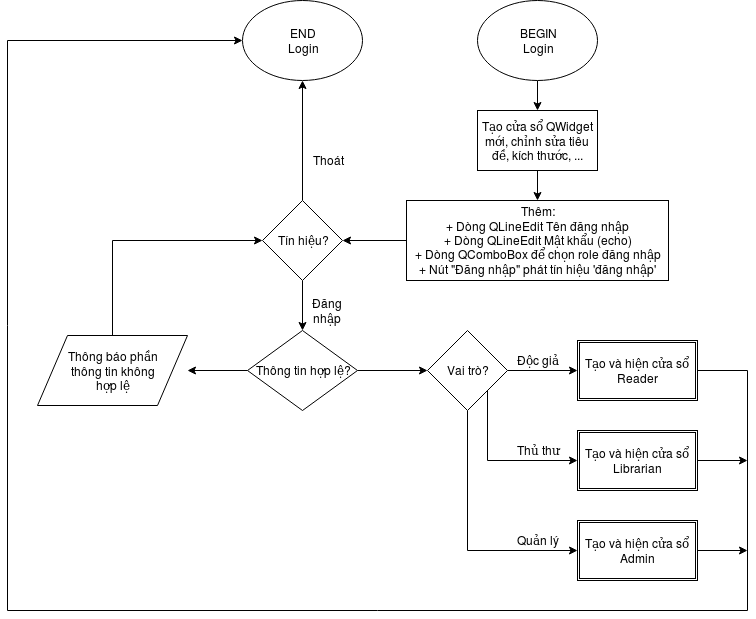
\includegraphics[scale=.5]{loginDiagram.png}
		\caption{Sơ đồ hoạt động của phần đăng nhập}
	\end{center}
\end{figure}
	\newpage \newpage 
\begin{figure}[h!]
	\begin{center}
		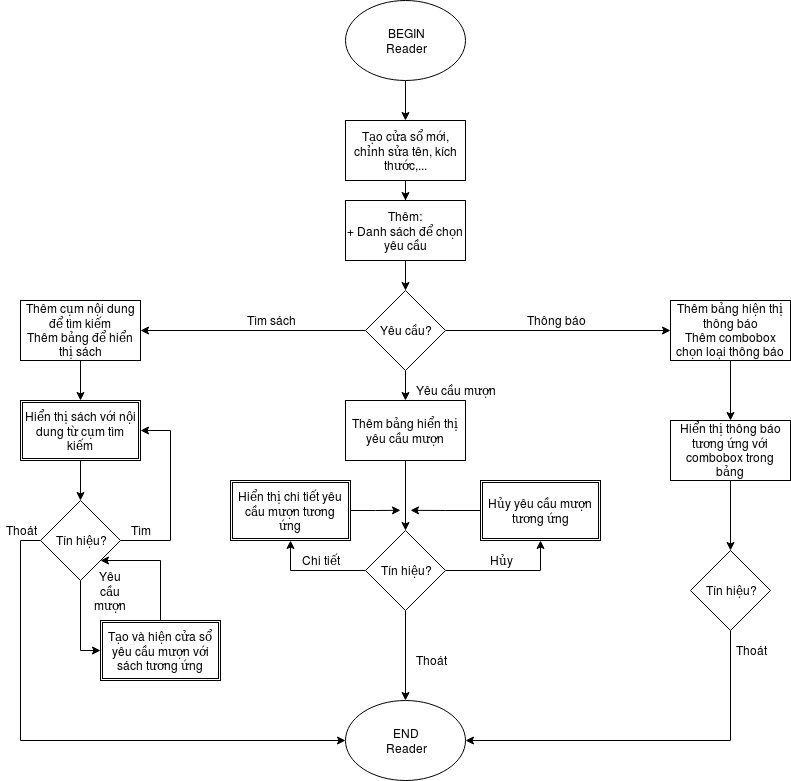
\includegraphics[scale=.5]{readerDiagram.png}
		\caption{Sơ đồ hoạt động của cửa sổ Reader}
	\end{center}
\end{figure}
	\newpage \newpage 
\begin{figure}[h!]
	\begin{center}
		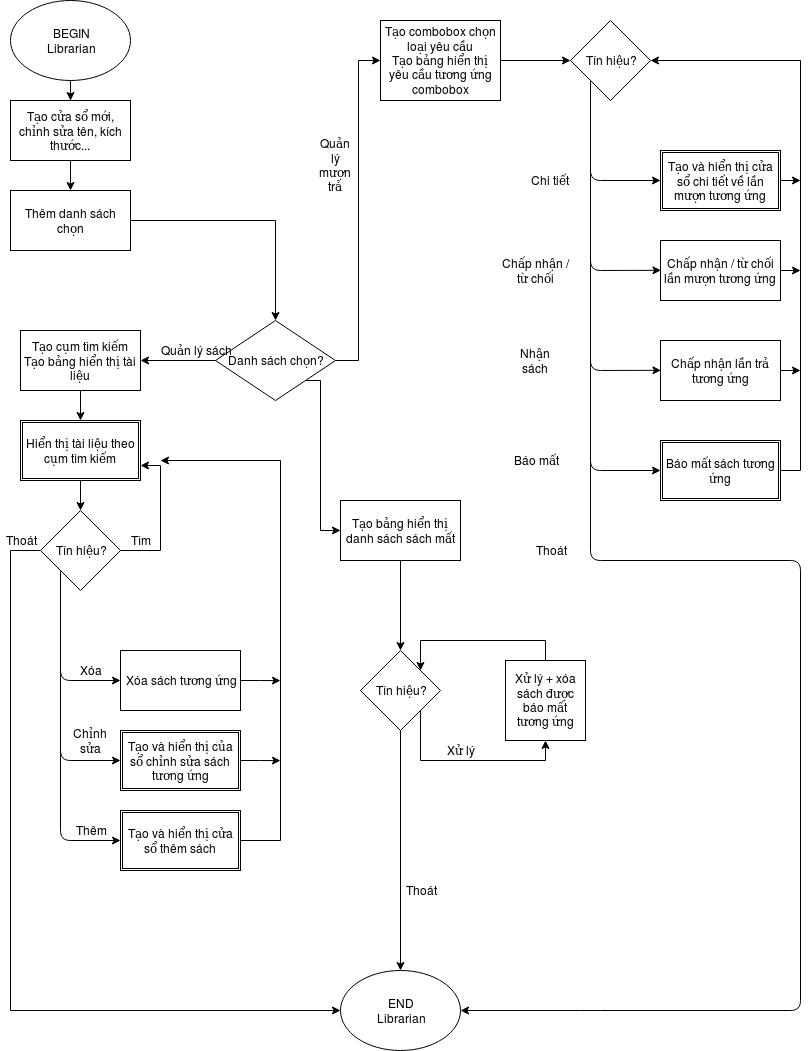
\includegraphics[scale=.5]{librarianDiagram.png}
		\caption{Sơ đồ hoạt động của cửa sổ Librarian}
	\end{center}
\end{figure}
	\newpage \newpage 
\begin{figure}[h!]
	\begin{center}
		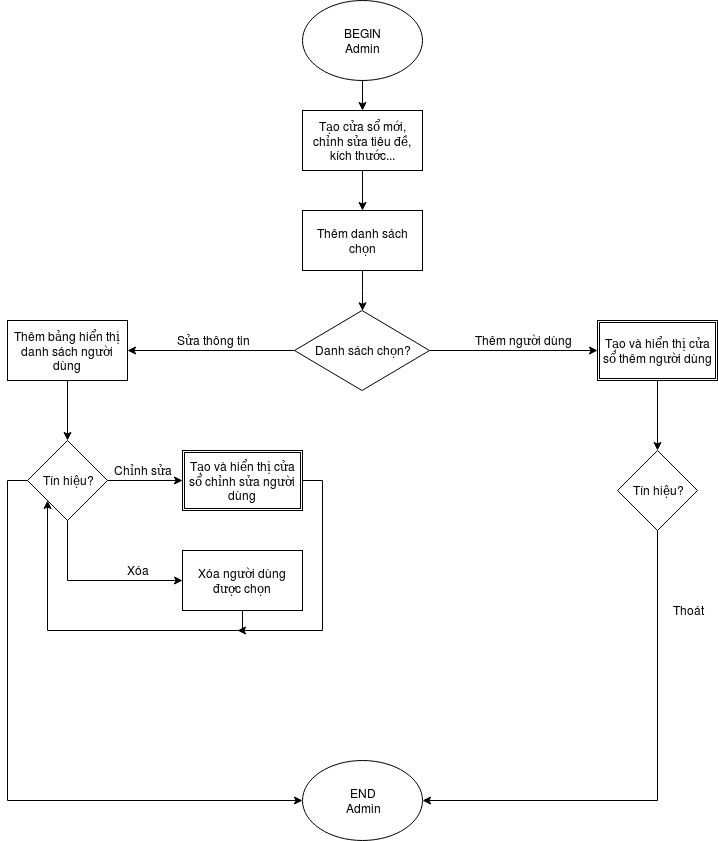
\includegraphics[scale=.5]{adminDiagram.png}
		\caption{Sơ đồ hoạt động của cửa sổ Admin}
	\end{center}
\end{figure}
	\newpage \newpage 
\subsection{Thiết kế giao diện}
Giao diện của phần mềm được thiết kế dưới sự hỗ trợ của IDE Qt\\
Các thư viện\& lớp sử dụng trên nền Qt:\\
\begin{itemize}
\item QtSql,QSqlDatabase, QSqlQuery: Các lớp hỗ trợ tương tác với dữ liệu từ cơ sở dữ l
\item QWidgets: Lớp đối tượng tương tác được trong GUI của Qt, bao gồm các cửa sổ, các tiêu đề, các box, textedit,...
\item QMainWindow: Lớp cửa sổ chính
\item QLabel, QLineEdit, QCheckBox,...: Các đối tượng tiêu đề, textedit,... trong GUI
\item QString, QDate, QList, QVector: Các lớp dữ liệu cơ bản được hỗ trợ tốt trong Qt
\item và rất nhiều lớp khác
\end{itemize}

\section{Tổ chức và quản lý mã nguồn trong quá trình quá triển}
Sơ đồ tổ chức code:\\
\begin{figure}[h!]
	\begin{center}
		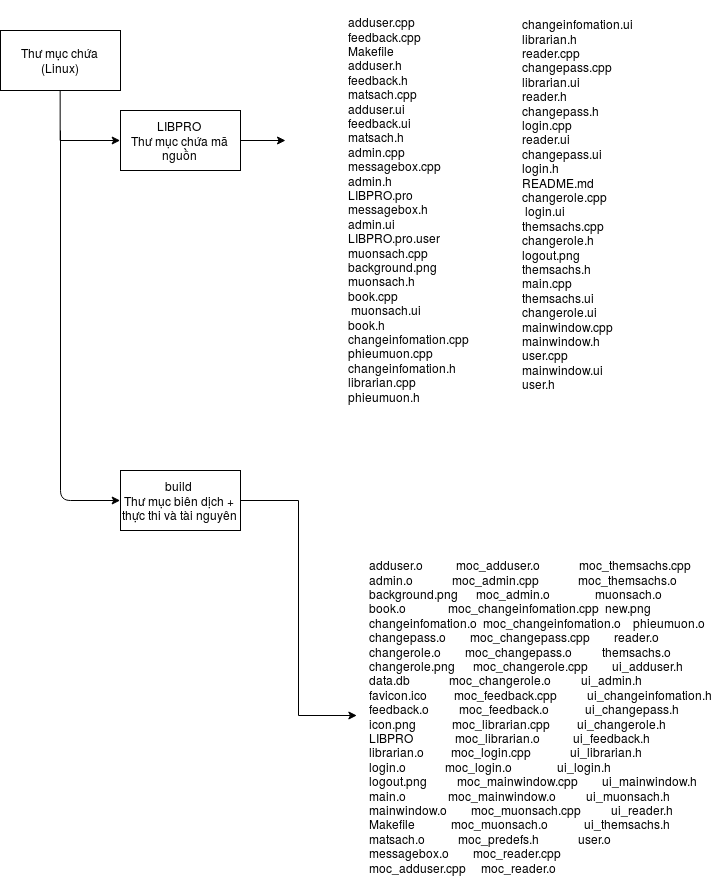
\includegraphics[scale=.5]{folderStructure.png}
		\caption{Cây tổ chức thư mục}
	\end{center}
\end{figure}
	\newpage \newpage 

Đường dẫn mã nguồn: \url{https://github.com/blackslender/LIBPRO.git}\\
Đường dân mã nguồn báo cáo: \url{https://github.com/blackslender/BCBTL2.git}\\
\section{Thu thập số liệu}
Các bước thu thập số liệu:\\
\begin{itemize}
\item 1. Xác định vấn đề cần nghiên cứu: Những yếu tố của phần mềm quản lí sách cua thư viện
\item 2. Thiết lập kế hoạch nghiên cứu:
\item 3. Tiến hành thu thập dữ liệu: Thu thập dữ liệu sẵn có trên website, tiến hành phỏng vấn các đối tượng liên quan
\item 4. Phân tích dữ liệu thu thập được.
\item 5. Phân bổ các kết quả phân tích.\\
<Trích \url{http://www.vnulib.edu.vn}>
\end{itemize}
Kết quả thu thập dữ liệu: phụ lục 9\\
\section{Kiểm tra phần mềm}
Nêu các testcases được thiết kế ra và kết quả kiểm tra. Lập bảng "checklist".

\section{Các tài liệu}
\subsection{Chú thích mã nguồn và định dạng}
Phần này cần tự đánh giá là có làm hay không và làm như thế nào thì có thể trích dẫn một hàm nào đó có đi kèm chú thích và được định dạng.
Trích dẫn phần xử lý cửa sổ chính: Phụ lục 9.3\\
\subsection{Tài liệu hổ trợ phát triển và nâng cấp}
Các nội dung liên quan để giúp người khác (không phải các thàn viên) theo tài liệu này thì có thể biên dịch dự án thành công và phát triển tiếp được.


kèm theo là các sơ đồ flowchart và mã giả cho các hàm quan trọng.

\subsection{Tài liệu hướng dẫn triển khai}
\subsection{Tài liệu hướng dẫn sử dụng phần mềm}


\section{Bảng tự đánh giá}
\subsection{Theo tiêu chí của giảng viên}
Viết một hoặc vài đoạn bàn về các kết quả đạt được với Bài tập lớn số 2 và những điểm chưa làm tốt (nếu có).

Phía cuối cùng của đoạn này, các thành viên cần tự đánh giá và cho điểm theo Bảng \ref{tb:rubrics}.

\begin{table}[h!]
	\centering
	\caption{Các tiêu chí chấm bài}
	\label{tb:rubrics}
	\begin{tabular}{|l|l|l|l|l|}
		\hline\hline
		\multicolumn{5}{|l|}{\textbf{Phần Bắt buộc}} \\
		\hline
		\textbf{STT} & \textbf{Tiêu chí} & \textbf{Báo cáo} & \textbf{Mã nguồn} & \textbf{C.Trình}\\
		\hline
		1. & Phân tích & 0.1 & &  \\ \hdashline
		2. & Thiết kế & 0.1 &&\\ \hdashline
		3. & Tổ chức mã nguồn & & 0.05 & \\ \hdashline
		4. & Thu thập số liệu & && \\\hdashline
		5. & Kiểm tra phần mềm & 0.025&& \\\hdashline
		6. & Lập tài liệu & 0.025& 0.05& \\\hdashline
		7. & Phân chia công việc và phối hợp & 0.025&& \\\hdashline
		8. & Báo cáo hoàn chỉnh và chuyên nghiệp &&& \\\hdashline
		9. & Sử dụng thành thạo nhập xuất màn hình & & & 0.1\\\hdashline
		10. & Sử dụng thành thạo nhập xuất tập tin &  & &  0.1\\\hdashline
		11. & Phát triển giải thuật phù hợp ($\in$ Báo cáo \& chương trình) & 0.025& & 0.4\\ \hdashline
		\multicolumn{2}{|r|}{\textbf{Tổng phần bắt buộc:}} &\textbf{0.3}& \textbf{0.1}& \textbf{0.6}\\
		
		\hline
		\multicolumn{5}{|l|}{\textbf{Phần cộng thêm}} \\
		\hline
		1. & Có sử dụng GUI &  && 0.1\\ \hdashline
		2. & Có sử dụng Git hay phần mềm tương đương & & 0.05& \\ \hdashline
		3. & Có sử dụng công cụ để thiết kế & 0.1 &&\\ \hdashline
		4. & Viết được Makefile &  & 0.05&\\ \hdashline
		5. & Có nhiều tính năng hay bổ sung & && 0.0 $\rightarrow$ 0.15 \\
		\hdashline
		\multicolumn{2}{|r|}{\textbf{Tổng phần cộng thêm:}} &\textbf{0.1}& \textbf{0.1}& \textbf{0.1 $\rightarrow$ 0.25}\\
		\hline
		\multicolumn{4}{|r|}{\textbf{Tổng toàn bộ}} & \textbf{1.3 $\rightarrow$ 1.45}\\
		
		
		
		
		
		\hline\hline
		
	\end{tabular}
	
\end{table}

\subsection{Những điểm khác}
Ngoài các tiêu chí cứng như trong Bảng \ref{tb:rubrics}, nếu nhóm thực hiện thấy những điểm mà nhóm đã nổ lực nhưng chưa được đánh giá trong các tiêu chí của giảng viên thì cũng có thể viết ra ở đây. Các thành viên có thể sẽ được cộng thêm điểm cho những cố gắng này.

Nếu không có thì nhóm nên xoá phần này khỏi báo cáo.




%%%%%%%%%%%%%%%%%%%%%%%%%%%%%%%%%
\addcontentsline{toc}{section}{Tài liệu tham khảo}
\begin{thebibliography}{99999}
\bibitem[tvtt]{tvtt} {Thư viện trung tâm, Đại học Quốc gia Tp.HCM: \url{http://www.vnulib.edu.vn/#1}}. Truy cập nhật dd/mm/yyyy.
\end{thebibliography} 
\newpage
\newpage
\section{Phụ lục}
\subsection{Các tên tài liệu được trích dẫn}
ID,TenSach,TacGia,NgayNhap,LoaiSach,GiaTien,SoLuong,NoiDung,NXB,DuocMuon\\
1,Giải tích 1,Nguyễn Đình Huy,2017-05-14,Giáo trình,"25,000",100,Sách mới,Đại học bách khoa,1\\
2,Vật lý 2,Trần Văn Lượng,2017-05-12,Giáo trình,"35,000",100,Nguyên vẹn,Đại học bách khoa,1\\
3,Hóa đại cương,Trần Văn B,2017-05-13,Giáo trình,"30,000",120,Nguyên vẹn,Đại học bách khoa,1\\
4,Đại số tuyến tính,Nguyễn Đình Huy,2017-05-13,Giáo trình,"25,000",110,Sách mới,ĐHQG-HCM ,1\\
6,Cơ lý thuyết,Vũ Duy Cường,2017-06-03,Giáo trình,"40,000",100,Sách mới,ĐHQG-HCM ,1\\
7,Bài tập hóa đại cương,Nguyễn Đức Chung,2017-06-03,Sách tham khảo,"30,000",150,Sách mới,ĐHQG-HCM ,1\\
8,Học sâu - Một cải tiến đơn giản có thể biến đổi việc dạy và học ở trường,KIERAN EGAN ,2017-06-23,Sách đại học ,"125,000",4,"""Dự án Học Sâu đã đem đến cho học sinh của chúng tôi một quan hệ hoàn toàn mới với việc học tập ở một độ sâu và phẩm chất đầy ngạc nhiên. Sau khi thấy dự án Học Sâu hoạt động thế nào trong các trường tại địa phương, tôi biết đây là một yếu tố quan trọng mà chúng ta còn thiếu. Nó chứng tỏ chính là mọi thứ mà chúng ta chưa tưởng tượng (cùng rất nhiều điều chúng ta chưa tưởng tượng tới) khi nghe nói tới kiến quan độc đáo của Kieran Egan"SHERI DUNTON - Giáo viên tiểu học Trường Tự chủ Corbett",ĐHQG-HCM ,1\\
5,Đại từ điển tiếng Việt,"Nguyễn Như Ý (Cb), Nguyễn Văn Khang, Vũ Quang Hào, Phan Xuân Thành ",2017-06-23,Sách công cụ ,"600,000 ",7,"Sách đáp ứng yêu cầu học tập và nghiên cứu của mọi giới người Việt Nam cũng như người nước ngoài muốn tìm hiểu, học tập và sử dụng tiếng Việt.",ĐHQG-HCM ,1\\
9,Cải cách và XD chương trình đào tạo kỹ thuật theo phương pháp tiếp cận CDIO,"Hồ Tấn Nhựt, Đoàn Thị Minh Trinh ",2017-06-23,Sách dịch,"170,000 ",4,"Quyển sách này đóng vai trò giới thiệu một phương pháp luận mới cho các ngành kỹ thuật bậc đại học nói riêng, và cho nền giáo dục bậc đại học và sau đại học ở Việt Nam nói chung để xây dựng và phát triển chương trình đào tạo.",ĐHQG-HCM ,1\\
10,Nguyên lý DESIGN thị giác,Nguyễn Hồng Hưng ,2017-06-23,Sách đại học ,"388,000 ",7,Sách dành cho sinh viên ngành kiến trúc. ,ĐHQG-HCM ,1\\
11,Marketing đương đại,"Ngô Bình, Nguyễn Khánh Trung ",2017-06-23,Sách chuyên khảo ,"90,000 ",4,Đối tượng là sinh viên kinh tế.,ĐHQG-HCM ,1\\
12,Các phương pháp nghiên cứu trong nhân học - Tiếp cận định tính và định lượng,H. Russel Bernard,2017-06-23,Sách dịch ,"80,000 ",7,"Sách dành cho sinh viên Khoa Nhân học, sinh viên ngành khoa học xã hội.",ĐHQG-HCM ,1\\
13,Hiện đại và động thái của truyền thống ở VN: Những các tiếp cận nhân học. Quyển 2,"Lương Văn Hy, Ngô Văn Lệ, Nguyễn Văn Tiệp, Phan Thị Yến Tuyết ",2017-06-23,Sách chuyên khảo ,"175,000 ",4,"Sách gồm nhiều nhiều bài từ hội thảo nhân học quốc tế về Việt Nam tại Bình Châu, 15-18/12/2007 do trường ĐH Khoa học Xã hội \& Nhân văn - Đại học Quốc gia Thành  phố Hồ Chí Minh, Việt Nam và Đại học Toronto, Canada đồng tổ chức.",ĐHQG-HCM ,1\\
14,Hiện đại và động thái của truyền thống ở VN: Những các tiếp cận nhân học. Quyển 1,"Lương Văn Hy, Ngô Văn Lệ, Nguyễn Văn Tiệp, Phan Thị Yến Tuyết ",2017-06-23,Sách chuyên khảo ,"145,000 ",7,"Sách gồm nhiều bài từ hội thảo nhân học quốc tế về Việt Nam tại Bình Châu, 15-18/12/2007 do trường Đại học Khoa học Xã hội \& Nhân văn - Đại học Quốc gia Thành phố Hồ Chí Minh, Việt Nam và Đại học Toroto, Canada đồng tổ chức.",ĐHQG-HCM ,1\\
15,Vùng ngập lũ đồng bằng sông Cửu Long - Hiện trạng và giải pháp,Nhiều tác giả ,2017-06-23,Sách chuyên khảo ,"127,000 ",7,"Quyển ""Vùng ngập lũ đồng bằng sông Cửu Long - Hiện trạng và giải pháp"" là tập hợp kết quả nghiên cứu thuộc đề tài độc lập cấp Nhà nước.",ĐHQG-HCM ,1\\
16,Văn học Việt Nam và Nhật Bản trong bối cảnh toàn cầu hóa,Nhiều tác giả ,2017-06-23,Sách chuyên khảo ,"300,000 ",13,"Toàn cầu hóa là một quá trình lịch sử lâu dài, diễn ra một cách thầm lặng nhưng không thể đảo ngược được giữa các quốc gia, các cộng đồng cư dân khác nhau để nhân loại có thể xích lại gần nhau trong mái nhà chung là trái đất. Từ cuối thế kỷ XX quá trình toàn cầu hóa được diễn ra với một tốc độ nhanh phi thường, khác hẳn trước kia. Toàn cầu hóa diễn ra ở mọi phương diện, từ kinh tế, xã hội đến khoa học, nghệ thuật. Đối với các dân tộc, trong đó có Việt Nam và Nhật Bản, toàn cầu hóa là cơ hội và thách thức. Trong bối cảnh toàn cầu hóa của thế kỷ XXI, nhiều vấn đề đặt ra đối với văn hóa, văn học của mỗi nước. Văn học Việt Nam và Nhật Bản sẽ phát triển thế nào, những yếu tố nào cần thay đổi, những giá trị mới nào cần phải tiếp thu trong quá trình ấy? Những người làm nghiên cứu, phê bình, giảng dạy văn học cần phải làm gì để góp phần vào sự phát triển đúng hướng của sáng tác và nghiên cứu, phê bình văn học trong tương lai? Việt Nam có thể học tập và rút kinh nghiệm gì từ con đường phát triển sáng tác, nghiên cứu, phê bình văn học Nhật Bản trong bối cảnh toàn cầu hóa đã và đang diễn ra?",NXB Đại Học Quốc Gia ,1\\
17,Cân bằng lợi ích giữa các bên trong hợp đồng nhượng quyền thương mại - Lý luận và thực tiễn,"Nguyễn Khánh Trung, Trần Thị Kim Phương ",2017-06-23,Sách chuyên khảo ,"75,000 ",4,"Nhượng quyền thương mại là một phương thức kinh doanh, trong đó bên nhượng quyền cho phép và yêu cầu bên nhận quyền tự tiến hành hoạt động mua bán hàng hóa, dịch vụ theo cách thức bên nhượng quyền quy định, gắn liền với nhãn hiệu, tên thương mại, bí quyết kinh doanh, ... của bên nhượng quyền. Tuy ở Việt Nam, hình thức này còn tương đối mới nhưng sức hấp dẫn và những ưu điểm của nó đã được khẳng định qua thực tế ở các nước phát triển trên thế giới. Trong thời gian tới, hình thức nhượng quyền thương mại được dự đoán sẽ phát triển bùng nổ ở nước ta, vì từ thời điểm từ năm 2014 là Việt Nam phải mở cửa hoàn toàn thị trường bán lẻ theo những điều khoản cam kết với WTO.",NXB Đại Học Quốc Gia ,1\\
18,Nhân học đại cương,Nhiều tác giả ,2017-06-23,Sách đại học ,"125,000 ",4,"Khoa Nhân học, Trường ĐH Khoa học Xã hội và Nhân văn – Đại học Quốc gia TP Hồ Chí Minh, được thành lập đến nay đã tròn 15 năm, đảm nhận đào tạo chương trình đại học và sau đại học. Cùng với hoạt động đào tạo và nghiên cứu khoa học, các cán bộ giảng dạy đã tiến hành biên soạn các tập bài giảng, giáo trình, dịch thuật nhiều tài liệu tham khảo từ tiếng nước ngoài để phục vụ công tác nghiên cứu, giảng dạy và học tập nhằm nâng cao chất lượng đào tạo. Một trong những công việc cấp bách của Khoa là biên soạn giáo trình ""Nhân học đại cương"" để giảng dạy cho sinh viên ngành nhân học cùng các ngành khoa học xã hội - nhân văn khác trong và ngoài trường. ",NXB Đại Học Quốc Gia ,1\\
19,Các phương pháp giải toán qua các kỳ thi Olympic,"Trần Nam Dũng (Cb), Võ Quốc Bá Cẩn, Lê Phúc Lữ ",2017-06-23,Sách tham khảo phổ thông ,"75,000 ",4,"Để giúp các em yêu thích môn toán tiếp cận với các đề thi và các chuyên đề Olympic toán học, các giảng viên Khoa Toán - Tin học, Trường ĐH Khoa học Tự nhiên, ĐHQG-HCM cùng các cộng sự đã thực hiện việc biên soạn cuốn ""Các phương pháp giải toán qua các kỳ thi Olympic"". ",NXB Đại Học Quốc Gia ,1\\
20,A Complete skill builder for the VNU-EPT TEST,Nhiều tác giả ,2017-06-23,Sách đại học ,"150,000 ",7,"Nằm trong khuôn khổ Đề án Ngoại ngữ Quốc gia Việt Nam 2020 của Bộ Giáo dục và Đào tạo, Đại học Quốc gia TP. HCM (ĐHQG-HCM) đang từng bước cải thiện việc giảng dạy, học tập và đánh giá các chương trình tiếng Anh ở các đơn vị thành viên trong vài năm trở lại đây. Riêng về mặt đánh giá, ĐHQG-HCM đã xây dựng Chứng chỉ tiếng Anh ĐHQG-HCM (English Proficiency Test - VNU-EPT) nhằm đánh giá khả năng ngôn ngữ của sinh viên dựa trên tiêu chuẩn của khung tham chiếu chung Châu Âu (CEFR). Bài thi VNU-EPT bao gồm bốn phần - Nghe, Đọc, Viết và Nói - và kéo dài khoảng ba giờ.",NXB Đại Học Quốc Gia ,1\\
21,Dịch vụ giáo dục quản lý \& kiểm định,Nguyễn Quang Toản ,2017-06-23,Sách công cụ ,"70,000 ",4,"Trong lĩnh vực giáo dục và đào tạo, tác giả đã đưa hệ thống quản lý chất lượng ISO vào hơn 30 trường đại học và cao đẳng của nước ta từ Bắc chí Nam để nâng cao chất lượng đào tạo và kiểm định chất lượng.",NXB Đại Học Quốc Gia ,1\\
22,Chủ nghĩa Hậu hiện đại và Phong trào tôn giáo mới ở Việt Nam và thế giới,Nhiều tác giả ,2017-06-23,Sách chuyên khảo ,"130,000",7,"Chủ nghĩa Hậu hiện đại và Phong trào tôn giáo mới xuất hiện vào khoảng nửa sau thế kỷ XIX và nhanh chóng trở thành những vấn đề phức tạp nhất và gây nhiều tranh cãi nhất trong cả lý luận và thực tiễn ỏ xã hội phương Tây hiện đại. Nếu như cuộc tranh luận về chủ nghĩa Hậu hiện đại của các lý thuyết gia hàng đầu hai bờ Đại Tây Dương được đẩy đến giới hạn cuối cùng của những phạm trù triết học, thì những quan niệm và sự hiện diện của tôn giáo mới lại vừa thể hiện tính gay gắt quyết liệt trong học thuật vừa là một thách thức đối với văn hóa tôn giáo truyền thống. Trên thực tế, Chủ nghĩa Hậu hiện đại và Phong trào tôn giáo mới đã có ảnh hưởng khá sâu rộng, tác động mạnh đến nhiều lĩnh vực của đời sống xã hội phương Tây hiện đại, đặc biệt là các lĩnh vực: triết học, tôn giáo, văn hóa, nghệ thuật, hội họa, kiến trúc.",NXB Đại Học Quốc Gia ,1\\
23,Chi tiết máy và ứng dụng tin học trong chi tiết máy,"Nguyễn Hữu Lộc, Lê Văn Uyển ",2017-06-23,Sách đại học ,"99,000",13,"Môn Chi tiết máy được đưa vào thi Olympic từ năm 2002, đến nay đã 12 năm. Môn Ứng dụng Tin học trong Cơ học (Chi tiết máy) đã được đưa vào từ năm 2011. Các kỳ thi này thúc đẩy phong trào dạy và học các môn Cơ học và Ứng dụng Tin học trong Cơ học tại các trường đại học và cao đẳng cả nước. Các em sinh viên đạt giải các kỳ thi này đã có nhiều thành công trong công tác, tiếp tục học tập nghiên cứu, nhiều em đã và đang làm công tác giảng dạy và nghiên cứu các trường đại học và các viện nghiên cứu ... . Nhiều em đã tiếp tục học cao hơn và được nhận bằng Tiến sĩ các trường danh tiếng nước ngoài ... . Đối với quý Thầy Cô, các kỳ thi Olympic này là cơ hội để nâng cao trình độ chuyên môn và phương pháp giảng dạy về các môn học, cũng như là dịp để trao đổi kinh nghiệm giảng dạy, thống nhất một số nội dung giảng dạy ...",NXB Đại Học Quốc Gia ,1\\
24,Tín ngưỡng thờ Mẫu ở Nam Bộ - Bản sắc và giá trị,Nhiều tác giả ,2017-06-23,Sách công cụ ,"340,000",4,"Hội thảo khoa học cấp quốc gia Tín ngưỡng thờ Mẫu ở Nam Bộ - bản sắc và giá trị (tháng 4 năm 2014) do Trường ĐH Khoa học Xã hội và Nhân văn – Đại học Quốc gia TP Hồ Chí Minh, Trung tâm Nghiên cứu và Bảo tồn Văn hóa tín ngưỡng Việt Nam, Sở Văn hóa Thể thao và Du lịch tỉnh An Giang và UBND TP. Châu Đốc tỉnh An Giang cùng phối hợp tổ chức là một diễn đàn quan trọng để các nhà nghiên cứu, các nhà quản lý, các nghệ nhân, giới thực hành sinh hoạt tín ngưỡng cùng trao đổi, phân tích, đánh giá những giá trị chung của tín ngưỡng thờ Mẫu ở Việt Nam nói chung cũng như nét đặc trưng mang tính bản sắc của vùng đất Nam Bộ.",NXB Đại Học Quốc Gia ,1\\
25,Chủ quyền Việt Nam trên Biển Đông và Hoàng Sa - Trường Sa,Nguyễn Đình Đầu ,2017-06-23,Sách công cụ ,"500,000 ",4,"Khi nói đến Biển Đông, người ta không thể không nhắc đến Hoàng Sa, Trường Sa. Trong tiềm thức của mỗi người dân Việt Nam, quần đảo Hoàng Sa, Trường Sa được coi là những vùng đất thiêng liêng của Tổ quốc. Đó là phần lãnh thổ mà cha ông tổ tiên ta từ thế hệ này sang thế hệ khác đã dày công khám phá, khai khẩn và đổ biết bao mồ hôi xương máu để bảo vệ, giữ gìn.",NXB Đại Học Quốc Gia ,1\\
26,FIVE PRACTICE TESTS FOR THE VNU-EPT,Nhiều tác giả ,2017-06-23,Sách đại học ,"120,000",7,"Nằm trong khuôn khổ Đề án Ngoại ngữ Quốc gia Việt Nam 2020 của Bộ Giáo dục và Đào tạo, Đại học Quốc gia TP. HCM (ĐHQG-HCM) đang từng bước cải thiện việc giảng dạy, học tập và đánh giá các chương trình tiếng Anh ở các đơn vị thành viên trong vài năm trở lại đây. Riêng về mặt đánh giá, ĐHQG-HCM đã xây dựng Chứng chỉ tiếng Anh ĐHQG-HCM (English Proficiency Test - VNU-EPT) nhằm đánh giá khả năng ngôn ngữ của sinh viên dựa trên tiêu chuẩn của khung tham chiếu chung Châu Âu (CEFR). Bài thi VNU-EPT bao gồm bốn phần - Nghe, Đọc, Viết và Nói - và kéo dài khoảng ba giờ. ",NXB Đại Học Quốc Gia ,1\\
27,Đại thi hào dân tộc - Danh nhân văn hóa Nguyễn Du,Nhiều tác giả ,2017-06-23,Sách tri thức ,"350,000",4,"Nguyễn Du (1765-1820) là nhà thơ vĩ đại của dân tộc. Truyện Kiều và các tác phẩm khác của ông được đánh giá là kiệt tác của văn học cổ điển Việt Nam, được nhân dân yêu quý, truyền tụng. Tác phẩm của ông được dịch ra rất nhiều thứ tiếng và được yêu mến trên thế giới. Tại phiên họp thứ 37 Đại hội đồng Tổ chức Giáo dục, Khoa học và Văn hóa Liên hiệp quốc (UNESCO) đã ra Nghị quyết số 37C/15 về việc kỷ niệm Nguyễn Du như một danh nhân văn hóa thế giới vào năm 2015 nhân dịp tròn 250 năm năm sinh của ông. Để vinh danh một đại thi hào dân tộc, đồng thời cũng là dịp để tìm hiểu rõ hơn về cuộc đời và những đóng góp của ông, Trường Đại học Khoa học Xã hội và Nhân văn - Đại học Quốc gia TPHCM quyết định tổ chức Hội thảo khoa học cấp Quốc gia ""Kỷ niệm 250 năm năm sinh Đại thi hào dân tộc Nguyễn Du"" vào ngày 23 tháng 12 năm 2015 tại Trường. Tập kỷ yếu này ra đời từ Hội thảo đó.",NXB Đại Học Quốc Gia ,1\\
28,Hôn nhân và gia đình của người Chu Ru,Võ Tấn Tú ,2017-06-23,Sách chuyên khảo ,"70,000 ",13,"Hôn nhân và gia đình từ lâu đã là đề tài nghiên cứu của các ngành khoa học như Nhân học/Dân tộc học, Xã hội học, Luật học, ... Hôn nhân và gia đình cũng là một lĩnh vực của đời sống xã hội có sức lôi cuốn những người hoạt động trong lĩnh vực văn hóa nghệ thuật. Nhiều tác phẩm văn học nghệ thuật có sức sống lâu dài nhờ gắn liền với đề tài hôn nhân và gia đình.",ĐHQG-HCM ,1\\
30,"Mối quan hệ giữa động lực làm việc và sự hài lòng công việc của cán bộ, công chức ở Việt Nam",Phạm Đức Chính (cb),2017-06-23,Sách chuyên khảo ,"174,000",7,"Thách thức với khu vực tư nhân hiện nay là phải tìm ra những đặc thù, bản sắc riêng cho mình từ những thành công và thất bại trong hoạt động nguồn nhân lực. Trong khi đó, mục đích hoạt động quản trị nguồn nhân lực ở khu vực công không chỉ dừng lại vậy. Thách thức sẽ lớn hơn rất nhiều, bởi các lý do: lượng biên chế lớn, hiệu quả kinh tế khó đo lường và tính chính danh về trách nhiệm trong cung cấp các dịch vụ công.",NXB Đại Học Quốc Gia ,1\\
31,Kế toán tài chính 2,Nguyễn Thị Khoa (cb),2017-06-23,Sách đại học ,"188,000",4,"Kế toán tài chính là môn học chuyên ngành cốt lõi được giảng dạy trong các chương trình đào tạo ngành Kế toán - Kiểm toán. Để tạo điều kiện cho sinh viên, giảng viên có tài liệu để học tập và nghiên cứu, Bộ môn Kế toán, khoa Kế toán - Kiểm toán, Trường ĐH Kinh tế-Luật thuộc ĐHQG TPHCM tổ chức biên soạn tài liệu tham khảo Kế toán tài chính nhằm hệ thống kiến thức và cập nhật những thay đổi mới nhất lĩnh vực kế toán tài chính phù hợp với xu hướng giảng dạy trong điều kiện hội nhập kế toán quốc tế.",NXB Đại Học Quốc Gia ,1\\
32,Việt Nam và Đông Nam Á trong bối cảnh toàn cầu hóa **,Nhiều tác giả ,2017-06-23,Sách chuyên khảo ,"320,000",4,"Ngày 31 tháng 12 năm 2015 đã mở ra một chương mới trong tiến trình phát triển của các nước Đông Nam Á, Cộng đồng ASEAN được chính thức ra đời. Bước khởi đầu đó mở ra một tương lai tươi sáng cho cộng đồng các quốc gia Đông Nam Á nhưng cũng dự báo không ít những khó khăn, thách thức trên con đường phát triển. Những kỳ vọng và sự trăn trở về con đường phát triển không chỉ ở những người lãnh đạo, những cộng đồng cư dân mà còn nơi các nhà khoa học từ các trường ĐH, các viện nghiên cứu ở Đông Nam Á và các nước khác. Cùng chia sẻ với các nhà lãnh đạo và các tầng lớp nhân dân về vấn đề hội nhập và phát triển, vừa qua Trường ĐH Khoa học Xã hội và Nhân văn thuộc ĐH QG-HCM đã phối hợp với Viện Nghiên cứu và Phát triển Phương Đông, ĐH Silpakorn - Thái Lan và Viện Dân tộc học tổ chức Hội thảo quốc tế ""VIỆT NAM - ĐÔNG NAM Á: HỘI NHẬP VÀ THÁCH THỨC"". Ban Tổ chức Hội thảo đã nhận được 82 tham luận của các nhà khoa học thuộc nhiều trường, viện gửi đến. Các bài viết của các tác giả thuộc nhiều lĩnh vực chuyên môn khác nhau, đề cập đến hầu hết các lĩnh vực lịch sử, kinh tế, văn hóa, xã hội được trình bày và thảo luận tại 5 biểu ban (5 chủ đề).",NXB Đại Học Quốc Gia ,1\\
33,Việt Nam và Đông Nam Á trong bối cảnh toàn cầu hóa *,Nhiều tác giả ,2017-06-23,Sách chuyên khảo ,"270,000",4,"Ngày 31 tháng 12 năm 2015 đã mở ra một chương mới trong tiến trình phát triển của các nước Đông Nam Á, Cộng đồng ASEAN được chính thức ra đời. Bước khởi đầu đó mở ra một tương lai tươi sáng cho cộng đồng các quốc gia Đông Nam Á nhưng cũng dự báo không ít những khó khăn, thách thức trên con đường phát triển. Những kỳ vọng và sự trăn trở về con đường phát triển không chỉ ở những người lãnh đạo, những cộng đồng cư dân mà còn nơi các nhà khoa học từ các trường ĐH, các viện nghiên cứu ở Đông Nam Á và các nước khác. Cùng chia sẻ với các nhà lãnh đạo và các tầng lớp nhân dân về vấn đề hội nhập và phát triển, vừa qua Trường ĐH Khoa học Xã hội và Nhân văn thuộc ĐH QG-HCM đã phối hợp với Viện Nghiên cứu và Phát triển Phương Đông, ĐH Silpakorn - Thái Lan và Viện Dân tộc học tổ chức Hội thảo quốc tế ""VIỆT NAM - ĐÔNG NAM Á: HỘI NHẬP VÀ THÁCH THỨC"". Ban Tổ chức Hội thảo đã nhận được 82 tham luận của các nhà khoa học thuộc nhiều trường, viện gửi đến. Các bài viết của các tác giả thuộc nhiều lĩnh vực chuyên môn khác nhau, đề cập đến hầu hết các lĩnh vực lịch sử, kinh tế, văn hóa, xã hội được trình bày và thảo luận tại 5 biểu ban (5 chủ đề).",NXB Đại Học Quốc Gia ,1\\
34,Tôn giáo mới - nhận thức và thực tế,Trương Văn Chung (cb),2017-06-23,Sách chuyên khảo ,"325,000",4,"Cuốn sách ""Tôn giáo mới - nhận thức và thực tế"" là kết quả từ quá trình nghiên cứu, tổng hợp tài liệu dịch thuật, các trang mạng, các phương tiện thông tin của tập thể tác giả từ nhiều năm và từ đề tài trọng điểm ĐHQG TPHCM ""Hiện tượng tôn giáo mới và những vấn đề về chính sách, công tác tôn giáo mới ở TPHCM"".",NXB Đại Học Quốc Gia ,1\\
35,Giáo trình Vi điều khiển,"Phan Đình Duy, Vũ Đức Lung, Lê Quang Minh ",2017-06-23,Sách đại học ,"23,000",37,"Xác định được tầm quan trọng của Vi điều khiển và nhu cầu của thị trường về lĩnh vực này rất lớn nên hậu hết các chương trình đào tạo lĩnh vực Điện tử - Kỹ thuật máy tính đều đưa ra nội dung vi điều khiển vào giảng dạy. Cuốn Giáo trình Vi điều khiển này nhằm giúp cho sinh viên tìm hiểu cấu trúc bên trong họ vi điều khiển cơ bản nhất, đó là họ vi điều khiển 8051, biết cách hoạt động của vi điều khiển và ứng dụng họ vi điều khiển này để thực hiện một số sản phẩm điều khiển trong thực tế.",NXB Đại Học Quốc Gia ,1\\
36,Giáo trình Phát triển phần mềm mã nguồn mở,"Vũ Thanh Nguyên, Nguyễn Công Hoan, Phan Trung Hiếu, Lê Đình Tuấn ",2017-06-23,Sách đại học ,"32,000",17,"Giáo trình ""Phát triển phần mềm mã nguồn mở"" sẽ giúp sinh viên có một cái nhìn tổng quan về lĩnh vực phát triển phần mềm mã nguồn mở, đồng thời trang bị cho sinh viên những kiến thức căn bản trong việc sử dụng phần mềm mã nguồn mở nói chung (như cách thức khảo sát, lựa chọn phần mềm mã nguồn mở cho phù hợp với nhu cầu học tập, công việc, ...) và các kỹ thuật cần thiết khi tham gia bảo trì, phát triển module mới hoặc phát triển một phần mềm mã nguồn mở hoàn toàn mới trên nhiều nền tảng công nghệ khác nhau.",ĐHQG-HCM ,1\\
37,Về khuôn mặt mới của Giáo dục Đại học Việt Nam,Phạm Phụ ,2017-06-23,Sách đại học ,"63,000",17,"Tác giả hy vọng người đọc có thêm được một số thông tin về Giáo dục Đại học Việt Nam, thông tin về một số xu thế phát triển Giáo dục Đại học trên thế giới và theo dõi được phần nào đó những tranh luận xung quanh các vấn đề về Giáo dục Đại học trong giai đoạn hiện nay.",ĐHQG-HCM ,1\\
38,Hướng dẫn ôn tập môn những nguyên lý cơ bản của chủ nghĩa Mác - Lênin,Nguyễn Văn Hiền ,2017-06-23,Sách đại học ,"25,000",37,"Tài liệu được biên soạn với nội dung kiến thức cơ bản, bảo đảm tính hệ thống và tuân thủ yêu cầu chương trình môn học NHỮNG NGUYÊN LÝ CƠ BẢN CỦA CHỦ NGHĨA MÁC - LÊNIN do Bộ trưởng Bộ giáo dục và Đào tạo ban hành và dựa trên GIÁO TRÌNH NHỮNG NGUYÊN LÝ CƠ BẢN CỦA CHỦ NGHĨA MÁC - LÊ NIN. Đồng thời, tài liệu có giới thiệu hệ thống câu hỏi ôn tập theo sát nội dung cơ bản sau mỗi chương nhằm định hướng cho sinh viên trong học tập và nghiên cứu.",ĐHQG-HCM ,1\\
39,Tư liệu nghiên cứu học tập Tư tưởng Hồ Chí Minh,Võ Văn Lộc ,,,"35,000",37,Tập tư liệu có một số đặc điểm sau:,ĐHQG-HCM ,1\\
\subsection{Makefile}
\begin{verbatim}
#############################################################################
# Makefile for building: LIBMANAGER
# Generated by qmake (3.0) (Qt 5.7.1)
# Project:  LIBMANAGER.pro
# Template: app
# Command: /usr/lib/x86_64-linux-gnu/qt5/bin/qmake QT+=sql QT+=widgets 
-o Makefile LIBMANAGER.pro
#############################################################################

MAKEFILE      = Makefile

####### Compiler, tools and options

CC            = gcc
CXX           = g++
DEFINES       = -DQT_NO_DEBUG -DQT_WIDGETS_LIB -DQT_GUI_LIB -DQT_SQL_LIB 
-DQT_CORE_LIB
CFLAGS        = -m64 -pipe -O2 -Wall -W -D_REENTRANT -fPIC $(DEFINES)
CXXFLAGS      = -m64 -pipe -O2 -Wall -W -D_REENTRANT -fPIC $(DEFINES)
INCPATH       = -I. -I. -isystem /usr/include/x86_64-linux-gnu/qt5 -isystem 
/usr/include/x86_64-linux-gnu/qt5/QtWidgets -isystem 
/usr/include/x86_64-linux-gnu/qt5/QtGui -isystem 
/usr/include/x86_64-linux-gnu/qt5/QtSql -isystem 
/usr/include/x86_64-linux-gnu/qt5/QtCore -I. -I. 
-I/usr/lib/x86_64-linux-gnu/qt5/mkspecs/linux-g++-64
QMAKE         = /usr/lib/x86_64-linux-gnu/qt5/bin/qmake
DEL_FILE      = rm -f
CHK_DIR_EXISTS= test -d
MKDIR         = mkdir -p
COPY          = cp -f
COPY_FILE     = cp -f
COPY_DIR      = cp -f -R
INSTALL_FILE  = install -m 644 -p
INSTALL_PROGRAM = install -m 755 -p
INSTALL_DIR   = cp -f -R
DEL_FILE      = rm -f
SYMLINK       = ln -f -s
DEL_DIR       = rmdir
MOVE          = mv -f
TAR           = tar -cf
COMPRESS      = gzip -9f
DISTNAME      = LIBMANAGER1.0.0
DISTDIR = /root/Downloads/LIBMANAGER/.tmp/LIBMANAGER1.0.0
LINK          = g++
LFLAGS        = -m64 -Wl,-O1
LIBS          = $(SUBLIBS) -L/usr/X11R6/lib64 -lQt5Widgets -lQt5Gui 
-lQt5Sql -lQt5Core -lGL -lpthread 
AR            = ar cqs
RANLIB        = 
SED           = sed
STRIP         = strip

####### Output directory

OBJECTS_DIR   = ./

####### Files

SOURCES       = adduser.cpp \
		admin.cpp \
		book.cpp \
		changeinfomation.cpp \
		changepass.cpp \
		librarian.cpp \
		login.cpp \
		main.cpp \
		mainwindow.cpp \
		matsach.cpp \
		messagebox.cpp \
		muonsach.cpp \
		phieumuon.cpp \
		reader.cpp \
		themsachs.cpp \
		user.cpp \
		changerole.cpp moc_adduser.cpp \
		moc_admin.cpp \
		moc_changeinfomation.cpp \
		moc_changepass.cpp \
		moc_librarian.cpp \
		moc_login.cpp \
		moc_mainwindow.cpp \
		moc_muonsach.cpp \
		moc_reader.cpp \
		moc_themsachs.cpp \
		moc_changerole.cpp
OBJECTS       = adduser.o \
		admin.o \
		book.o \
		changeinfomation.o \
		changepass.o \
		librarian.o \
		login.o \
		main.o \
		mainwindow.o \
		matsach.o \
		messagebox.o \
		muonsach.o \
		phieumuon.o \
		reader.o \
		themsachs.o \
		user.o \
		changerole.o \
		moc_adduser.o \
		moc_admin.o \
		moc_changeinfomation.o \
		moc_changepass.o \
		moc_librarian.o \
		moc_login.o \
		moc_mainwindow.o \
		moc_muonsach.o \
		moc_reader.o \
		moc_themsachs.o \
		moc_changerole.o
DIST    = /usr/lib/x86_64-linux-gnu/qt5/mkspecs/features/spec_pre.prf \
		/usr/lib/x86_64-linux-gnu/qt5/mkspecs/common/unix.conf \
		/usr/lib/x86_64-linux-gnu/qt5/mkspecs/common/linux.conf \
		/usr/lib/x86_64-linux-gnu/qt5/mkspecs/common/sanitize.conf \
		/usr/lib/x86_64-linux-gnu/qt5/mkspecs/common/gcc-base.conf \
		/usr/lib/x86_64-linux-gnu/qt5/mkspecs/common/gcc-base-unix.conf \
		/usr/lib/x86_64-linux-gnu/qt5/mkspecs/common/g++-base.conf \
		/usr/lib/x86_64-linux-gnu/qt5/mkspecs/common/g++-unix.conf \
		/usr/lib/x86_64-linux-gnu/qt5/mkspecs/qconfig.pri \
		/usr/lib/x86_64-linux-gnu/qt5/mkspecs/modules/qt_lib_bootstrap_private.pri \
		/usr/lib/x86_64-linux-gnu/qt5/mkspecs/modules/qt_lib_concurrent.pri \
		/usr/lib/x86_64-linux-gnu/qt5/mkspecs/modules/qt_lib_concurrent_private.pri \
		/usr/lib/x86_64-linux-gnu/qt5/mkspecs/modules/qt_lib_core.pri \
		/usr/lib/x86_64-linux-gnu/qt5/mkspecs/modules/qt_lib_core_private.pri \
		/usr/lib/x86_64-linux-gnu/qt5/mkspecs/modules/qt_lib_dbus.pri \
		/usr/lib/x86_64-linux-gnu/qt5/mkspecs/modules/qt_lib_dbus_private.pri \
		/usr/lib/x86_64-linux-gnu/qt5/mkspecs/modules/qt_lib_eglfs_device_lib_private.pri \
		/usr/lib/x86_64-linux-gnu/qt5/mkspecs/modules/qt_lib_eglfs_kms_support_private.pri \
		/usr/lib/x86_64-linux-gnu/qt5/mkspecs/modules/qt_lib_gui.pri \
		/usr/lib/x86_64-linux-gnu/qt5/mkspecs/modules/qt_lib_gui_private.pri \
		/usr/lib/x86_64-linux-gnu/qt5/mkspecs/modules/qt_lib_network.pri \
		/usr/lib/x86_64-linux-gnu/qt5/mkspecs/modules/qt_lib_network_private.pri \
		/usr/lib/x86_64-linux-gnu/qt5/mkspecs/modules/qt_lib_opengl.pri \
		/usr/lib/x86_64-linux-gnu/qt5/mkspecs/modules/qt_lib_opengl_private.pri \
		/usr/lib/x86_64-linux-gnu/qt5/mkspecs/modules/qt_lib_openglextensions.pri \
		/usr/lib/x86_64-linux-gnu/qt5/mkspecs/modules/qt_lib_openglextensions_private.pri \
		/usr/lib/x86_64-linux-gnu/qt5/mkspecs/modules/qt_lib_platformsupport_private.pri \
		/usr/lib/x86_64-linux-gnu/qt5/mkspecs/modules/qt_lib_printsupport.pri \
		/usr/lib/x86_64-linux-gnu/qt5/mkspecs/modules/qt_lib_printsupport_private.pri \
		/usr/lib/x86_64-linux-gnu/qt5/mkspecs/modules/qt_lib_qml.pri \
		/usr/lib/x86_64-linux-gnu/qt5/mkspecs/modules/qt_lib_qmltest.pri \
		/usr/lib/x86_64-linux-gnu/qt5/mkspecs/modules/qt_lib_quick.pri \
		/usr/lib/x86_64-linux-gnu/qt5/mkspecs/modules/qt_lib_quickwidgets.pri \
		/usr/lib/x86_64-linux-gnu/qt5/mkspecs/modules/qt_lib_sql.pri \
		/usr/lib/x86_64-linux-gnu/qt5/mkspecs/modules/qt_lib_sql_private.pri \
		/usr/lib/x86_64-linux-gnu/qt5/mkspecs/modules/qt_lib_testlib.pri \
		/usr/lib/x86_64-linux-gnu/qt5/mkspecs/modules/qt_lib_testlib_private.pri \
		/usr/lib/x86_64-linux-gnu/qt5/mkspecs/modules/qt_lib_widgets.pri \
		/usr/lib/x86_64-linux-gnu/qt5/mkspecs/modules/qt_lib_widgets_private.pri \
		/usr/lib/x86_64-linux-gnu/qt5/mkspecs/modules/qt_lib_xcb_qpa_lib_private.pri \
		/usr/lib/x86_64-linux-gnu/qt5/mkspecs/modules/qt_lib_xml.pri \
		/usr/lib/x86_64-linux-gnu/qt5/mkspecs/modules/qt_lib_xml_private.pri \
		/usr/lib/x86_64-linux-gnu/qt5/mkspecs/features/qt_functions.prf \
		/usr/lib/x86_64-linux-gnu/qt5/mkspecs/features/qt_config.prf \
		/usr/lib/x86_64-linux-gnu/qt5/mkspecs/linux-g++-64/qmake.conf \
		/usr/lib/x86_64-linux-gnu/qt5/mkspecs/features/spec_post.prf \
		.qmake.stash \
		/usr/lib/x86_64-linux-gnu/qt5/mkspecs/features/exclusive_builds.prf \
		/usr/lib/x86_64-linux-gnu/qt5/mkspecs/features/toolchain.prf \
		/usr/lib/x86_64-linux-gnu/qt5/mkspecs/features/default_pre.prf \
		/usr/lib/x86_64-linux-gnu/qt5/mkspecs/features/resolve_config.prf \
		/usr/lib/x86_64-linux-gnu/qt5/mkspecs/features/default_post.prf \
		/usr/lib/x86_64-linux-gnu/qt5/mkspecs/features/warn_on.prf \
		/usr/lib/x86_64-linux-gnu/qt5/mkspecs/features/qt.prf \
		/usr/lib/x86_64-linux-gnu/qt5/mkspecs/features/resources.prf \
		/usr/lib/x86_64-linux-gnu/qt5/mkspecs/features/moc.prf \
		/usr/lib/x86_64-linux-gnu/qt5/mkspecs/features/unix/opengl.prf \
		/usr/lib/x86_64-linux-gnu/qt5/mkspecs/features/uic.prf \
		/usr/lib/x86_64-linux-gnu/qt5/mkspecs/features/unix/thread.prf \
		/usr/lib/x86_64-linux-gnu/qt5/mkspecs/features/file_copies.prf \
		/usr/lib/x86_64-linux-gnu/qt5/mkspecs/features/testcase_targets.prf \
		/usr/lib/x86_64-linux-gnu/qt5/mkspecs/features/exceptions.prf \
		/usr/lib/x86_64-linux-gnu/qt5/mkspecs/features/yacc.prf \
		/usr/lib/x86_64-linux-gnu/qt5/mkspecs/features/lex.prf \
		LIBMANAGER.pro adduser.h \
		admin.h \
		book.h \
		changeinfomation.h \
		changepass.h \
		librarian.h \
		login.h \
		mainwindow.h \
		matsach.h \
		messagebox.h \
		muonsach.h \
		phieumuon.h \
		reader.h \
		themsachs.h \
		ui_adduser.h \
		ui_admin.h \
		ui_changeinfomation.h \
		ui_changepass.h \
		ui_librarian.h \
		ui_login.h \
		ui_mainwindow.h \
		ui_muonsach.h \
		ui_reader.h \
		ui_themsachs.h \
		user.h \
		changerole.h adduser.cpp \
		admin.cpp \
		book.cpp \
		changeinfomation.cpp \
		changepass.cpp \
		librarian.cpp \
		login.cpp \
		main.cpp \
		mainwindow.cpp \
		matsach.cpp \
		messagebox.cpp \
		muonsach.cpp \
		phieumuon.cpp \
		reader.cpp \
		themsachs.cpp \
		user.cpp \
		changerole.cpp
QMAKE_TARGET  = LIBMANAGER
DESTDIR       = 
TARGET        = LIBMANAGER


first: all
####### Build rules

$(TARGET): ui_adduser.h ui_admin.h ui_changeinfomation.h 
ui_changepass.h ui_librarian.h ui_login.h ui_mainwindow.h 
ui_muonsach.h ui_reader.h ui_themsachs.h ui_changerole.h $(OBJECTS)  
	$(LINK) $(LFLAGS) -o $(TARGET) $(OBJECTS) $(OBJCOMP) $(LIBS)

Makefile: LIBMANAGER.pro /usr/lib/x86_64-linux-gnu/qt5/mkspecs/linux-g++-64/qmake.conf 
/usr/lib/x86_64-linux-gnu/qt5/mkspecs/features/spec_pre.prf \
		/usr/lib/x86_64-linux-gnu/qt5/mkspecs/common/unix.conf \
		/usr/lib/x86_64-linux-gnu/qt5/mkspecs/common/linux.conf \
		/usr/lib/x86_64-linux-gnu/qt5/mkspecs/common/sanitize.conf \
		/usr/lib/x86_64-linux-gnu/qt5/mkspecs/common/gcc-base.conf \
		/usr/lib/x86_64-linux-gnu/qt5/mkspecs/common/gcc-base-unix.conf \
		/usr/lib/x86_64-linux-gnu/qt5/mkspecs/common/g++-base.conf \
		/usr/lib/x86_64-linux-gnu/qt5/mkspecs/common/g++-unix.conf \
		/usr/lib/x86_64-linux-gnu/qt5/mkspecs/qconfig.pri \
		/usr/lib/x86_64-linux-gnu/qt5/mkspecs/modules/qt_lib_bootstrap_private.pri \
		/usr/lib/x86_64-linux-gnu/qt5/mkspecs/modules/qt_lib_concurrent.pri \
		/usr/lib/x86_64-linux-gnu/qt5/mkspecs/modules/qt_lib_concurrent_private.pri \
		/usr/lib/x86_64-linux-gnu/qt5/mkspecs/modules/qt_lib_core.pri \
		/usr/lib/x86_64-linux-gnu/qt5/mkspecs/modules/qt_lib_core_private.pri \
		/usr/lib/x86_64-linux-gnu/qt5/mkspecs/modules/qt_lib_dbus.pri \
		/usr/lib/x86_64-linux-gnu/qt5/mkspecs/modules/qt_lib_dbus_private.pri \
		/usr/lib/x86_64-linux-gnu/qt5/mkspecs/modules/qt_lib_eglfs_device_lib_private.pri \
		/usr/lib/x86_64-linux-gnu/qt5/mkspecs/modules/qt_lib_eglfs_kms_support_private.pri \
		/usr/lib/x86_64-linux-gnu/qt5/mkspecs/modules/qt_lib_gui.pri \
		/usr/lib/x86_64-linux-gnu/qt5/mkspecs/modules/qt_lib_gui_private.pri \
		/usr/lib/x86_64-linux-gnu/qt5/mkspecs/modules/qt_lib_network.pri \
		/usr/lib/x86_64-linux-gnu/qt5/mkspecs/modules/qt_lib_network_private.pri \
		/usr/lib/x86_64-linux-gnu/qt5/mkspecs/modules/qt_lib_opengl.pri \
		/usr/lib/x86_64-linux-gnu/qt5/mkspecs/modules/qt_lib_opengl_private.pri \
		/usr/lib/x86_64-linux-gnu/qt5/mkspecs/modules/qt_lib_openglextensions.pri \
		/usr/lib/x86_64-linux-gnu/qt5/mkspecs/modules/qt_lib_openglextensions_private.pri \
		/usr/lib/x86_64-linux-gnu/qt5/mkspecs/modules/qt_lib_platformsupport_private.pri \
		/usr/lib/x86_64-linux-gnu/qt5/mkspecs/modules/qt_lib_printsupport.pri \
		/usr/lib/x86_64-linux-gnu/qt5/mkspecs/modules/qt_lib_printsupport_private.pri \
		/usr/lib/x86_64-linux-gnu/qt5/mkspecs/modules/qt_lib_qml.pri \
		/usr/lib/x86_64-linux-gnu/qt5/mkspecs/modules/qt_lib_qmltest.pri \
		/usr/lib/x86_64-linux-gnu/qt5/mkspecs/modules/qt_lib_quick.pri \
		/usr/lib/x86_64-linux-gnu/qt5/mkspecs/modules/qt_lib_quickwidgets.pri \
		/usr/lib/x86_64-linux-gnu/qt5/mkspecs/modules/qt_lib_sql.pri \
		/usr/lib/x86_64-linux-gnu/qt5/mkspecs/modules/qt_lib_sql_private.pri \
		/usr/lib/x86_64-linux-gnu/qt5/mkspecs/modules/qt_lib_testlib.pri \
		/usr/lib/x86_64-linux-gnu/qt5/mkspecs/modules/qt_lib_testlib_private.pri \
		/usr/lib/x86_64-linux-gnu/qt5/mkspecs/modules/qt_lib_widgets.pri \
		/usr/lib/x86_64-linux-gnu/qt5/mkspecs/modules/qt_lib_widgets_private.pri \
		/usr/lib/x86_64-linux-gnu/qt5/mkspecs/modules/qt_lib_xcb_qpa_lib_private.pri \
		/usr/lib/x86_64-linux-gnu/qt5/mkspecs/modules/qt_lib_xml.pri \
		/usr/lib/x86_64-linux-gnu/qt5/mkspecs/modules/qt_lib_xml_private.pri \
		/usr/lib/x86_64-linux-gnu/qt5/mkspecs/features/qt_functions.prf \
		/usr/lib/x86_64-linux-gnu/qt5/mkspecs/features/qt_config.prf \
		/usr/lib/x86_64-linux-gnu/qt5/mkspecs/linux-g++-64/qmake.conf \
		/usr/lib/x86_64-linux-gnu/qt5/mkspecs/features/spec_post.prf \
		.qmake.stash \
		/usr/lib/x86_64-linux-gnu/qt5/mkspecs/features/exclusive_builds.prf \
		/usr/lib/x86_64-linux-gnu/qt5/mkspecs/features/toolchain.prf \
		/usr/lib/x86_64-linux-gnu/qt5/mkspecs/features/default_pre.prf \
		/usr/lib/x86_64-linux-gnu/qt5/mkspecs/features/resolve_config.prf \
		/usr/lib/x86_64-linux-gnu/qt5/mkspecs/features/default_post.prf \
		/usr/lib/x86_64-linux-gnu/qt5/mkspecs/features/warn_on.prf \
		/usr/lib/x86_64-linux-gnu/qt5/mkspecs/features/qt.prf \
		/usr/lib/x86_64-linux-gnu/qt5/mkspecs/features/resources.prf \
		/usr/lib/x86_64-linux-gnu/qt5/mkspecs/features/moc.prf \
		/usr/lib/x86_64-linux-gnu/qt5/mkspecs/features/unix/opengl.prf \
		/usr/lib/x86_64-linux-gnu/qt5/mkspecs/features/uic.prf \
		/usr/lib/x86_64-linux-gnu/qt5/mkspecs/features/unix/thread.prf \
		/usr/lib/x86_64-linux-gnu/qt5/mkspecs/features/file_copies.prf \
		/usr/lib/x86_64-linux-gnu/qt5/mkspecs/features/testcase_targets.prf \
		/usr/lib/x86_64-linux-gnu/qt5/mkspecs/features/exceptions.prf \
		/usr/lib/x86_64-linux-gnu/qt5/mkspecs/features/yacc.prf \
		/usr/lib/x86_64-linux-gnu/qt5/mkspecs/features/lex.prf \
		LIBMANAGER.pro \
		/usr/lib/x86_64-linux-gnu/libQt5Widgets.prl \
		/usr/lib/x86_64-linux-gnu/libQt5Gui.prl \
		/usr/lib/x86_64-linux-gnu/libQt5Sql.prl \
		/usr/lib/x86_64-linux-gnu/libQt5Core.prl
	$(QMAKE) QT+=sql QT+=widgets -o Makefile LIBMANAGER.pro
/usr/lib/x86_64-linux-gnu/qt5/mkspecs/features/spec_pre.prf:
/usr/lib/x86_64-linux-gnu/qt5/mkspecs/common/unix.conf:
/usr/lib/x86_64-linux-gnu/qt5/mkspecs/common/linux.conf:
/usr/lib/x86_64-linux-gnu/qt5/mkspecs/common/sanitize.conf:
/usr/lib/x86_64-linux-gnu/qt5/mkspecs/common/gcc-base.conf:
/usr/lib/x86_64-linux-gnu/qt5/mkspecs/common/gcc-base-unix.conf:
/usr/lib/x86_64-linux-gnu/qt5/mkspecs/common/g++-base.conf:
/usr/lib/x86_64-linux-gnu/qt5/mkspecs/common/g++-unix.conf:
/usr/lib/x86_64-linux-gnu/qt5/mkspecs/qconfig.pri:
/usr/lib/x86_64-linux-gnu/qt5/mkspecs/modules/qt_lib_bootstrap_private.pri:
/usr/lib/x86_64-linux-gnu/qt5/mkspecs/modules/qt_lib_concurrent.pri:
/usr/lib/x86_64-linux-gnu/qt5/mkspecs/modules/qt_lib_concurrent_private.pri:
/usr/lib/x86_64-linux-gnu/qt5/mkspecs/modules/qt_lib_core.pri:
/usr/lib/x86_64-linux-gnu/qt5/mkspecs/modules/qt_lib_core_private.pri:
/usr/lib/x86_64-linux-gnu/qt5/mkspecs/modules/qt_lib_dbus.pri:
/usr/lib/x86_64-linux-gnu/qt5/mkspecs/modules/qt_lib_dbus_private.pri:
/usr/lib/x86_64-linux-gnu/qt5/mkspecs/modules/qt_lib_eglfs_device_lib_private.pri:
/usr/lib/x86_64-linux-gnu/qt5/mkspecs/modules/qt_lib_eglfs_kms_support_private.pri:
/usr/lib/x86_64-linux-gnu/qt5/mkspecs/modules/qt_lib_gui.pri:
/usr/lib/x86_64-linux-gnu/qt5/mkspecs/modules/qt_lib_gui_private.pri:
/usr/lib/x86_64-linux-gnu/qt5/mkspecs/modules/qt_lib_network.pri:
/usr/lib/x86_64-linux-gnu/qt5/mkspecs/modules/qt_lib_network_private.pri:
/usr/lib/x86_64-linux-gnu/qt5/mkspecs/modules/qt_lib_opengl.pri:
/usr/lib/x86_64-linux-gnu/qt5/mkspecs/modules/qt_lib_opengl_private.pri:
/usr/lib/x86_64-linux-gnu/qt5/mkspecs/modules/qt_lib_openglextensions.pri:
/usr/lib/x86_64-linux-gnu/qt5/mkspecs/modules/qt_lib_openglextensions_private.pri:
/usr/lib/x86_64-linux-gnu/qt5/mkspecs/modules/qt_lib_platformsupport_private.pri:
/usr/lib/x86_64-linux-gnu/qt5/mkspecs/modules/qt_lib_printsupport.pri:
/usr/lib/x86_64-linux-gnu/qt5/mkspecs/modules/qt_lib_printsupport_private.pri:
/usr/lib/x86_64-linux-gnu/qt5/mkspecs/modules/qt_lib_qml.pri:
/usr/lib/x86_64-linux-gnu/qt5/mkspecs/modules/qt_lib_qmltest.pri:
/usr/lib/x86_64-linux-gnu/qt5/mkspecs/modules/qt_lib_quick.pri:
/usr/lib/x86_64-linux-gnu/qt5/mkspecs/modules/qt_lib_quickwidgets.pri:
/usr/lib/x86_64-linux-gnu/qt5/mkspecs/modules/qt_lib_sql.pri:
/usr/lib/x86_64-linux-gnu/qt5/mkspecs/modules/qt_lib_sql_private.pri:
/usr/lib/x86_64-linux-gnu/qt5/mkspecs/modules/qt_lib_testlib.pri:
/usr/lib/x86_64-linux-gnu/qt5/mkspecs/modules/qt_lib_testlib_private.pri:
/usr/lib/x86_64-linux-gnu/qt5/mkspecs/modules/qt_lib_widgets.pri:
/usr/lib/x86_64-linux-gnu/qt5/mkspecs/modules/qt_lib_widgets_private.pri:
/usr/lib/x86_64-linux-gnu/qt5/mkspecs/modules/qt_lib_xcb_qpa_lib_private.pri:
/usr/lib/x86_64-linux-gnu/qt5/mkspecs/modules/qt_lib_xml.pri:
/usr/lib/x86_64-linux-gnu/qt5/mkspecs/modules/qt_lib_xml_private.pri:
/usr/lib/x86_64-linux-gnu/qt5/mkspecs/features/qt_functions.prf:
/usr/lib/x86_64-linux-gnu/qt5/mkspecs/features/qt_config.prf:
/usr/lib/x86_64-linux-gnu/qt5/mkspecs/linux-g++-64/qmake.conf:
/usr/lib/x86_64-linux-gnu/qt5/mkspecs/features/spec_post.prf:
.qmake.stash:
/usr/lib/x86_64-linux-gnu/qt5/mkspecs/features/exclusive_builds.prf:
/usr/lib/x86_64-linux-gnu/qt5/mkspecs/features/toolchain.prf:
/usr/lib/x86_64-linux-gnu/qt5/mkspecs/features/default_pre.prf:
/usr/lib/x86_64-linux-gnu/qt5/mkspecs/features/resolve_config.prf:
/usr/lib/x86_64-linux-gnu/qt5/mkspecs/features/default_post.prf:
/usr/lib/x86_64-linux-gnu/qt5/mkspecs/features/warn_on.prf:
/usr/lib/x86_64-linux-gnu/qt5/mkspecs/features/qt.prf:
/usr/lib/x86_64-linux-gnu/qt5/mkspecs/features/resources.prf:
/usr/lib/x86_64-linux-gnu/qt5/mkspecs/features/moc.prf:
/usr/lib/x86_64-linux-gnu/qt5/mkspecs/features/unix/opengl.prf:
/usr/lib/x86_64-linux-gnu/qt5/mkspecs/features/uic.prf:
/usr/lib/x86_64-linux-gnu/qt5/mkspecs/features/unix/thread.prf:
/usr/lib/x86_64-linux-gnu/qt5/mkspecs/features/file_copies.prf:
/usr/lib/x86_64-linux-gnu/qt5/mkspecs/features/testcase_targets.prf:
/usr/lib/x86_64-linux-gnu/qt5/mkspecs/features/exceptions.prf:
/usr/lib/x86_64-linux-gnu/qt5/mkspecs/features/yacc.prf:
/usr/lib/x86_64-linux-gnu/qt5/mkspecs/features/lex.prf:
LIBMANAGER.pro:
/usr/lib/x86_64-linux-gnu/libQt5Widgets.prl:
/usr/lib/x86_64-linux-gnu/libQt5Gui.prl:
/usr/lib/x86_64-linux-gnu/libQt5Sql.prl:
/usr/lib/x86_64-linux-gnu/libQt5Core.prl:
qmake: FORCE
	@$(QMAKE) QT+=sql QT+=widgets -o Makefile LIBMANAGER.pro

qmake_all: FORCE


all: Makefile $(TARGET)

dist: distdir FORCE
	(cd `dirname $(DISTDIR)` && $(TAR) $(DISTNAME).tar $(DISTNAME) 
	&& $(COMPRESS) $(DISTNAME).tar) && $(MOVE) `dirname $(DISTDIR)`/$(DISTNAME).tar.gz . 
	&& $(DEL_FILE) -r $(DISTDIR)

distdir: FORCE
	@test -d $(DISTDIR) || mkdir -p $(DISTDIR)
	$(COPY_FILE) --parents $(DIST) $(DISTDIR)/
	$(COPY_FILE) --parents adduser.h admin.h book.h changeinfomation.h 
	changepass.h librarian.h login.h mainwindow.h matsach.h messagebox.h 
	muonsach.h phieumuon.h reader.h themsachs.h ui_adduser.h ui_admin.h 
	ui_changeinfomation.h ui_changepass.h ui_librarian.h ui_login.h 
	ui_mainwindow.h ui_muonsach.h ui_reader.h ui_themsachs.h user.h 
	changerole.h $(DISTDIR)/
	$(COPY_FILE) --parents adduser.cpp admin.cpp book.cpp changeinfomation.cpp 
	changepass.cpp librarian.cpp login.cpp main.cpp mainwindow.cpp matsach.cpp messagebox.cpp 
	muonsach.cpp phieumuon.cpp reader.cpp themsachs.cpp user.cpp changerole.cpp $(DISTDIR)/
	$(COPY_FILE) --parents adduser.ui admin.ui changeinfomation.ui changepass.ui librarian.ui 
	login.ui mainwindow.ui muonsach.ui reader.ui themsachs.ui changerole.ui $(DISTDIR)/


clean: compiler_clean 
	-$(DEL_FILE) $(OBJECTS)
	-$(DEL_FILE) *~ core *.core


distclean: clean 
	-$(DEL_FILE) $(TARGET) 
	-$(DEL_FILE) .qmake.stash
	-$(DEL_FILE) Makefile


####### Sub-libraries

mocclean: compiler_moc_header_clean compiler_moc_source_clean

mocables: compiler_moc_header_make_all compiler_moc_source_make_all

check: first

benchmark: first

compiler_rcc_make_all:
compiler_rcc_clean:
compiler_moc_header_make_all: moc_adduser.cpp moc_admin.cpp 
moc_changeinfomation.cpp moc_changepass.cpp moc_librarian.cpp moc_login.cpp 
moc_mainwindow.cpp moc_muonsach.cpp moc_reader.cpp moc_themsachs.cpp moc_changerole.cpp
compiler_moc_header_clean:
	-$(DEL_FILE) moc_adduser.cpp moc_admin.cpp moc_changeinfomation.cpp 
	moc_changepass.cpp moc_librarian.cpp moc_login.cpp moc_mainwindow.cpp 
	moc_muonsach.cpp moc_reader.cpp moc_themsachs.cpp moc_changerole.cpp
moc_adduser.cpp: user.h \
		adduser.h \
		/usr/lib/x86_64-linux-gnu/qt5/bin/moc
	/usr/lib/x86_64-linux-gnu/qt5/bin/moc $(DEFINES) 
	-I/usr/lib/x86_64-linux-gnu/qt5/mkspecs/linux-g++-64 
	-I/root/Downloads/LIBMANAGER
		root/Downloads/LIBMANAGER 
	-I/usr/include/x86_64-linux-gnu/qt5
		usr/include/x86_64-linux-gnu/qt5/QtWidgets 
	-I/usr/include/x86_64-linux-gnu/qt5/QtGui
		usr/include/x86_64-linux-gnu/qt5/QtSql 
	-I/usr/include/x86_64-linux-gnu/qt5/QtCore
		usr/include/c++/6 
	-I/usr/include/x86_64-linux-gnu/c++/6
		usr/include/c++/6/backward 
	-I/usr/lib/gcc/x86_64-linux-gnu/6/include
		usr/local/include 
	-I/usr/lib/gcc/x86_64-linux-gnu/6/include-fixed
		usr/include/x86_64-linux-gnu 
	-I/usr/include adduser.h -o moc_adduser.cpp

moc_admin.cpp: user.h \
		admin.h \
		/usr/lib/x86_64-linux-gnu/qt5/bin/moc
	/usr/lib/x86_64-linux-gnu/qt5/bin/moc $(DEFINES) 
	-I/usr/lib/x86_64-linux-gnu/qt5/mkspecs/linux-g++-64 
	-I/root/Downloads/LIBMANAGER
		root/Downloads/LIBMANAGER 
	-I/usr/include/x86_64-linux-gnu/qt5
		usr/include/x86_64-linux-gnu/qt5/QtWidgets 
	-I/usr/include/x86_64-linux-gnu/qt5/QtGui
		usr/include/x86_64-linux-gnu/qt5/QtSql 
	-I/usr/include/x86_64-linux-gnu/qt5/QtCore
		usr/include/c++/6 
	-I/usr/include/x86_64-linux-gnu/c++/6
		usr/include/c++/6/backward 
	-I/usr/lib/gcc/x86_64-linux-gnu/6/include
		usr/local/include 
	-I/usr/lib/gcc/x86_64-linux-gnu/6/include-fixed
		usr/include/x86_64-linux-gnu 
	-I/usr/include admin.h -o moc_admin.cpp

moc_changeinfomation.cpp: user.h \
		changeinfomation.h \
		/usr/lib/x86_64-linux-gnu/qt5/bin/moc
	/usr/lib/x86_64-linux-gnu/qt5/bin/moc $(DEFINES) 
	-I/usr/lib/x86_64-linux-gnu/qt5/mkspecs/linux-g++-64
		root/Downloads/LIBMANAGER 
	-I/root/Downloads/LIBMANAGER
		usr/include/x86_64-linux-gnu/qt5 
	-I/usr/include/x86_64-linux-gnu/qt5/QtWidgets
		usr/include/x86_64-linux-gnu/qt5/QtGui 
	-I/usr/include/x86_64-linux-gnu/qt5/QtSql
		usr/include/x86_64-linux-gnu/qt5/QtCore 
	-I/usr/include/c++/6
		usr/include/x86_64-linux-gnu/c++/6
		usr/include/c++/6/backward 
	-I/usr/lib/gcc/x86_64-linux-gnu/6/include
		usr/local/include 
	-I/usr/lib/gcc/x86_64-linux-gnu/6/include-fixed
		usr/include/x86_64-linux-gnu 
	-I/usr/include changeinfomation.h -o moc_changeinfomation.cpp

moc_changepass.cpp: user.h \
		changepass.h \
		/usr/lib/x86_64-linux-gnu/qt5/bin/moc
	/usr/lib/x86_64-linux-gnu/qt5/bin/moc $(DEFINES) 
	-I/usr/lib/x86_64-linux-gnu/qt5/mkspecs/linux-g++-64
		root/Downloads/LIBMANAGER 
	-I/root/Downloads/LIBMANAGER
		usr/include/x86_64-linux-gnu/qt5 
	-I/usr/include/x86_64-linux-gnu/qt5/QtWidgets
		usr/include/x86_64-linux-gnu/qt5/QtGui 
	-I/usr/include/x86_64-linux-gnu/qt5/QtSql
		usr/include/x86_64-linux-gnu/qt5/QtCore 
	-I/usr/include/c++/6
		usr/include/x86_64-linux-gnu/c++/6
		usr/include/c++/6/backward 
	-I/usr/lib/gcc/x86_64-linux-gnu/6/include
		usr/local/include 
	-I/usr/lib/gcc/x86_64-linux-gnu/6/include-fixed
		usr/include/x86_64-linux-gnu 
	-I/usr/include changepass.h -o moc_changepass.cpp

moc_librarian.cpp: user.h \
		librarian.h \
		/usr/lib/x86_64-linux-gnu/qt5/bin/moc
	/usr/lib/x86_64-linux-gnu/qt5/bin/moc $(DEFINES)
		usr/lib/x86_64-linux-gnu/qt5/mkspecs/linux-g++-64
		root/Downloads/LIBMANAGER
		root/Downloads/LIBMANAGER
		usr/include/x86_64-linux-gnu/qt5
		usr/include/x86_64-linux-gnu/qt5/QtWidgets
		usr/include/x86_64-linux-gnu/qt5/QtGui
		usr/include/x86_64-linux-gnu/qt5/QtSql
		usr/include/x86_64-linux-gnu/qt5/QtCore
		usr/include/c++/6
		usr/include/x86_64-linux-gnu/c++/6
		usr/include/c++/6/backward
		usr/lib/gcc/x86_64-linux-gnu/6/include
		usr/local/include
		usr/lib/gcc/x86_64-linux-gnu/6/include-fixed
		usr/include/x86_64-linux-gnu
		usr/include librarian.h -o moc_librarian.cpp

moc_login.cpp: user.h \
		login.h \
		/usr/lib/x86_64-linux-gnu/qt5/bin/moc
	/usr/lib/x86_64-linux-gnu/qt5/bin/moc $(DEFINES)
		usr/lib/x86_64-linux-gnu/qt5/mkspecs/linux-g++-64
		root/Downloads/LIBMANAGER
		root/Downloads/LIBMANAGER
		usr/include/x86_64-linux-gnu/qt5
		usr/include/x86_64-linux-gnu/qt5/QtWidgets
		usr/include/x86_64-linux-gnu/qt5/QtGui
		usr/include/x86_64-linux-gnu/qt5/QtSql
		usr/include/x86_64-linux-gnu/qt5/QtCore
		usr/include/c++/6
		usr/include/x86_64-linux-gnu/c++/6
		usr/include/c++/6/backward
		usr/lib/gcc/x86_64-linux-gnu/6/include
		usr/local/include
		usr/lib/gcc/x86_64-linux-gnu/6/include-fixed
		usr/include/x86_64-linux-gnu
		usr/include login.h -o moc_login.cpp

moc_mainwindow.cpp: user.h \
		login.h \
		reader.h \
		mainwindow.h \
		/usr/lib/x86_64-linux-gnu/qt5/bin/moc
	/usr/lib/x86_64-linux-gnu/qt5/bin/moc $(DEFINES)
		usr/lib/x86_64-linux-gnu/qt5/mkspecs/linux-g++-64
		root/Downloads/LIBMANAGER
		root/Downloads/LIBMANAGER
		usr/include/x86_64-linux-gnu/qt5
		usr/include/x86_64-linux-gnu/qt5/QtWidgets
		usr/include/x86_64-linux-gnu/qt5/QtGui
		usr/include/x86_64-linux-gnu/qt5/QtSql
		usr/include/x86_64-linux-gnu/qt5/QtCore
		usr/include/c++/6
		usr/include/x86_64-linux-gnu/c++/6
		usr/include/c++/6/backward
		usr/lib/gcc/x86_64-linux-gnu/6/include
		usr/local/include
		usr/lib/gcc/x86_64-linux-gnu/6/include-fixed
		usr/include/x86_64-linux-gnu
		usr/include mainwindow.h -o moc_mainwindow.cpp

moc_muonsach.cpp: book.h \
		muonsach.h \
		/usr/lib/x86_64-linux-gnu/qt5/bin/moc
	/usr/lib/x86_64-linux-gnu/qt5/bin/moc $(DEFINES)
		usr/lib/x86_64-linux-gnu/qt5/mkspecs/linux-g++-64
		root/Downloads/LIBMANAGER
		root/Downloads/LIBMANAGER
		usr/include/x86_64-linux-gnu/qt5
		usr/include/x86_64-linux-gnu/qt5/QtWidgets
		usr/include/x86_64-linux-gnu/qt5/QtGui
		usr/include/x86_64-linux-gnu/qt5/QtSql
		usr/include/x86_64-linux-gnu/qt5/QtCore
		usr/include/c++/6
		usr/include/x86_64-linux-gnu/c++/6
		usr/include/c++/6/backward
		usr/lib/gcc/x86_64-linux-gnu/6/include
		usr/local/include
		usr/lib/gcc/x86_64-linux-gnu/6/include-fixed
		usr/include/x86_64-linux-gnu
		usr/include muonsach.h -o moc_muonsach.cpp

moc_reader.cpp: user.h \
		reader.h \
		/usr/lib/x86_64-linux-gnu/qt5/bin/moc
	/usr/lib/x86_64-linux-gnu/qt5/bin/moc $(DEFINES)
		usr/lib/x86_64-linux-gnu/qt5/mkspecs/linux-g++-64
		root/Downloads/LIBMANAGER
		root/Downloads/LIBMANAGER
		usr/include/x86_64-linux-gnu/qt5
		usr/include/x86_64-linux-gnu/qt5/QtWidgets
		usr/include/x86_64-linux-gnu/qt5/QtGui
		usr/include/x86_64-linux-gnu/qt5/QtSql
		usr/include/x86_64-linux-gnu/qt5/QtCore
		usr/include/c++/6
		usr/include/x86_64-linux-gnu/c++/6
		usr/include/c++/6/backward
		usr/lib/gcc/x86_64-linux-gnu/6/include
		usr/local/include
		usr/lib/gcc/x86_64-linux-gnu/6/include-fixed
		usr/include/x86_64-linux-gnu
		usr/include reader.h -o moc_reader.cpp

moc_themsachs.cpp: book.h \
		themsachs.h \
		/usr/lib/x86_64-linux-gnu/qt5/bin/moc
	/usr/lib/x86_64-linux-gnu/qt5/bin/moc $(DEFINES)
		usr/lib/x86_64-linux-gnu/qt5/mkspecs/linux-g++-64
		root/Downloads/LIBMANAGER
		root/Downloads/LIBMANAGER
		usr/include/x86_64-linux-gnu/qt5
		usr/include/x86_64-linux-gnu/qt5/QtWidgets
		usr/include/x86_64-linux-gnu/qt5/QtGui
		usr/include/x86_64-linux-gnu/qt5/QtSql
		usr/include/x86_64-linux-gnu/qt5/QtCore
		usr/include/c++/6
		usr/include/x86_64-linux-gnu/c++/6
		usr/include/c++/6/backward
		usr/lib/gcc/x86_64-linux-gnu/6/include
		usr/local/include
		usr/lib/gcc/x86_64-linux-gnu/6/include-fixed
		usr/include/x86_64-linux-gnu
		usr/include themsachs.h -o moc_themsachs.cpp

moc_changerole.cpp: user.h \
		changerole.h \
		/usr/lib/x86_64-linux-gnu/qt5/bin/moc
	/usr/lib/x86_64-linux-gnu/qt5/bin/moc $(DEFINES)
		usr/lib/x86_64-linux-gnu/qt5/mkspecs/linux-g++-64
		root/Downloads/LIBMANAGER
		root/Downloads/LIBMANAGER
		usr/include/x86_64-linux-gnu/qt5
		usr/include/x86_64-linux-gnu/qt5/QtWidgets
		usr/include/x86_64-linux-gnu/qt5/QtGui
		usr/include/x86_64-linux-gnu/qt5/QtSql
		usr/include/x86_64-linux-gnu/qt5/QtCore
		usr/include/c++/6
		usr/include/x86_64-linux-gnu/c++/6
		usr/include/c++/6/backward
		usr/lib/gcc/x86_64-linux-gnu/6/include
		usr/local/include
		usr/lib/gcc/x86_64-linux-gnu/6/include-fixed
		usr/include/x86_64-linux-gnu
		usr/include changerole.h -o moc_changerole.cpp

compiler_moc_source_make_all:
compiler_moc_source_clean:
compiler_uic_make_all: ui_adduser.h ui_admin.h ui_changeinfomation.h 
ui_changepass.h ui_librarian.h ui_login.h ui_mainwindow.h ui_muonsach.h 
ui_reader.h ui_themsachs.h ui_changerole.h
compiler_uic_clean:
	-$(DEL_FILE) ui_adduser.h ui_admin.h ui_changeinfomation.h 
	ui_changepass.h ui_librarian.h ui_login.h ui_mainwindow.h ui_muonsach.h 
	ui_reader.h ui_themsachs.h ui_changerole.h
ui_adduser.h: adduser.ui \
		/usr/lib/x86_64-linux-gnu/qt5/bin/uic
	/usr/lib/x86_64-linux-gnu/qt5/bin/uic adduser.ui -o ui_adduser.h

ui_admin.h: admin.ui \
		/usr/lib/x86_64-linux-gnu/qt5/bin/uic
	/usr/lib/x86_64-linux-gnu/qt5/bin/uic admin.ui -o ui_admin.h

ui_changeinfomation.h: changeinfomation.ui \
		/usr/lib/x86_64-linux-gnu/qt5/bin/uic
	/usr/lib/x86_64-linux-gnu/qt5/bin/uic changeinfomation.ui -o 
	ui_changeinfomation.h

ui_changepass.h: changepass.ui \
		/usr/lib/x86_64-linux-gnu/qt5/bin/uic
	/usr/lib/x86_64-linux-gnu/qt5/bin/uic changepass.ui -o ui_changepass.h

ui_librarian.h: librarian.ui \
		/usr/lib/x86_64-linux-gnu/qt5/bin/uic
	/usr/lib/x86_64-linux-gnu/qt5/bin/uic librarian.ui -o ui_librarian.h

ui_login.h: login.ui \
		/usr/lib/x86_64-linux-gnu/qt5/bin/uic
	/usr/lib/x86_64-linux-gnu/qt5/bin/uic login.ui -o ui_login.h

ui_mainwindow.h: mainwindow.ui \
		/usr/lib/x86_64-linux-gnu/qt5/bin/uic
	/usr/lib/x86_64-linux-gnu/qt5/bin/uic mainwindow.ui -o ui_mainwindow.h

ui_muonsach.h: muonsach.ui \
		/usr/lib/x86_64-linux-gnu/qt5/bin/uic
	/usr/lib/x86_64-linux-gnu/qt5/bin/uic muonsach.ui -o ui_muonsach.h

ui_reader.h: reader.ui \
		/usr/lib/x86_64-linux-gnu/qt5/bin/uic
	/usr/lib/x86_64-linux-gnu/qt5/bin/uic reader.ui -o ui_reader.h

ui_themsachs.h: themsachs.ui \
		/usr/lib/x86_64-linux-gnu/qt5/bin/uic
	/usr/lib/x86_64-linux-gnu/qt5/bin/uic themsachs.ui -o ui_themsachs.h

ui_changerole.h: changerole.ui \
		/usr/lib/x86_64-linux-gnu/qt5/bin/uic
	/usr/lib/x86_64-linux-gnu/qt5/bin/uic changerole.ui -o ui_changerole.h

compiler_yacc_decl_make_all:
compiler_yacc_decl_clean:
compiler_yacc_impl_make_all:
compiler_yacc_impl_clean:
compiler_lex_make_all:
compiler_lex_clean:
compiler_clean: compiler_moc_header_clean compiler_uic_clean 

####### Compile

adduser.o: adduser.cpp adduser.h \
		user.h \
		ui_adduser.h
	$(CXX) -c $(CXXFLAGS) $(INCPATH) -o adduser.o adduser.cpp

admin.o: admin.cpp admin.h \
		user.h \
		ui_admin.h \
		adduser.h
	$(CXX) -c $(CXXFLAGS) $(INCPATH) -o admin.o admin.cpp

book.o: book.cpp book.h \
		phieumuon.h
	$(CXX) -c $(CXXFLAGS) $(INCPATH) -o book.o book.cpp

changeinfomation.o: changeinfomation.cpp changeinfomation.h \
		user.h \
		ui_changeinfomation.h
	$(CXX) -c $(CXXFLAGS) $(INCPATH) -o changeinfomation.o changeinfomation.cpp

changepass.o: changepass.cpp changepass.h \
		user.h \
		ui_changepass.h
	$(CXX) -c $(CXXFLAGS) $(INCPATH) -o changepass.o changepass.cpp

librarian.o: librarian.cpp librarian.h \
		user.h \
		ui_librarian.h \
		phieumuon.h \
		muonsach.h \
		book.h \
		themsachs.h \
		matsach.h
	$(CXX) -c $(CXXFLAGS) $(INCPATH) -o librarian.o librarian.cpp

login.o: login.cpp login.h \
		user.h \
		ui_login.h \
		reader.h
	$(CXX) -c $(CXXFLAGS) $(INCPATH) -o login.o login.cpp

main.o: main.cpp mainwindow.h \
		user.h \
		login.h \
		reader.h
	$(CXX) -c $(CXXFLAGS) $(INCPATH) -o main.o main.cpp

mainwindow.o: mainwindow.cpp mainwindow.h \
		user.h \
		login.h \
		reader.h \
		ui_mainwindow.h \
		changeinfomation.h \
		changepass.h \
		admin.h \
		librarian.h \
		phieumuon.h \
		changerole.h \
		book.h
	$(CXX) -c $(CXXFLAGS) $(INCPATH) -o mainwindow.o mainwindow.cpp

matsach.o: matsach.cpp matsach.h
	$(CXX) -c $(CXXFLAGS) $(INCPATH) -o matsach.o matsach.cpp

messagebox.o: messagebox.cpp messagebox.h
	$(CXX) -c $(CXXFLAGS) $(INCPATH) -o messagebox.o messagebox.cpp

muonsach.o: muonsach.cpp muonsach.h \
		book.h \
		phieumuon.h \
		ui_muonsach.h
	$(CXX) -c $(CXXFLAGS) $(INCPATH) -o muonsach.o muonsach.cpp

phieumuon.o: phieumuon.cpp phieumuon.h \
		book.h
	$(CXX) -c $(CXXFLAGS) $(INCPATH) -o phieumuon.o phieumuon.cpp

reader.o: reader.cpp reader.h \
		user.h \
		ui_reader.h \
		muonsach.h \
		book.h \
		phieumuon.h
	$(CXX) -c $(CXXFLAGS) $(INCPATH) -o reader.o reader.cpp

themsachs.o: themsachs.cpp themsachs.h \
		book.h \
		ui_themsachs.h \
		messagebox.h
	$(CXX) -c $(CXXFLAGS) $(INCPATH) -o themsachs.o themsachs.cpp

user.o: user.cpp user.h
	$(CXX) -c $(CXXFLAGS) $(INCPATH) -o user.o user.cpp

changerole.o: changerole.cpp changerole.h \
		user.h \
		ui_changerole.h
	$(CXX) -c $(CXXFLAGS) $(INCPATH) -o changerole.o changerole.cpp

moc_adduser.o: moc_adduser.cpp 
	$(CXX) -c $(CXXFLAGS) $(INCPATH) -o moc_adduser.o moc_adduser.cpp

moc_admin.o: moc_admin.cpp 
	$(CXX) -c $(CXXFLAGS) $(INCPATH) -o moc_admin.o moc_admin.cpp

moc_changeinfomation.o: moc_changeinfomation.cpp 
	$(CXX) -c $(CXXFLAGS) $(INCPATH) -o moc_changeinfomation.o moc_changeinfomation.cpp

moc_changepass.o: moc_changepass.cpp 
	$(CXX) -c $(CXXFLAGS) $(INCPATH) -o moc_changepass.o moc_changepass.cpp

moc_librarian.o: moc_librarian.cpp 
	$(CXX) -c $(CXXFLAGS) $(INCPATH) -o moc_librarian.o moc_librarian.cpp

moc_login.o: moc_login.cpp 
	$(CXX) -c $(CXXFLAGS) $(INCPATH) -o moc_login.o moc_login.cpp

moc_mainwindow.o: moc_mainwindow.cpp 
	$(CXX) -c $(CXXFLAGS) $(INCPATH) -o moc_mainwindow.o moc_mainwindow.cpp

moc_muonsach.o: moc_muonsach.cpp 
	$(CXX) -c $(CXXFLAGS) $(INCPATH) -o moc_muonsach.o moc_muonsach.cpp

moc_reader.o: moc_reader.cpp 
	$(CXX) -c $(CXXFLAGS) $(INCPATH) -o moc_reader.o moc_reader.cpp

moc_themsachs.o: moc_themsachs.cpp 
	$(CXX) -c $(CXXFLAGS) $(INCPATH) -o moc_themsachs.o moc_themsachs.cpp

moc_changerole.o: moc_changerole.cpp 
	$(CXX) -c $(CXXFLAGS) $(INCPATH) -o moc_changerole.o moc_changerole.cpp

####### Install

install:  FORCE

uninstall:  FORCE

FORCE:

\end{verbatim}
\subsection{Trích dẫn code mẫu phần xử lý cửa sổ chính}
\begin{lstlisting}
#include "mainwindow.h"
#include "ui_mainwindow.h"
#include "changeinfomation.h"
#include <QDebug>
#include "reader.h"
#include "changepass.h"
#include "admin.h"
#include "librarian.h"
#include "phieumuon.h"
#include "changerole.h"
#include <QWidget>
#include <QtWidgets>
#include <QMdiSubWindow>
#include <QLayout>
#include <book.h>
#include "feedback.h"
#include <QDir>
MainWindow::MainWindow(QWidget *parent) :
    QMainWindow(parent),
    ui(new Ui::MainWindow)
{
    //Khoi tao form
    ui->setupUi(this);
    //Load Database
    db=new QSqlDatabase(QSqlDatabase::addDatabase("QSQLITE"));
    db->setDatabaseName(DIR("data.db"));
    db->open();
    //Tao vung MDI
    mdi=new QMdiArea();
    QImage background(DIR("background.png"));
    mdi->setBackground(background);
    user=new USER();
    //Show toolbar
    showToolbar();
    //Bat dau show form login
    LoginShow();
    Logined=false;
    setCentralWidget(mdi);
    this->setWindowTitle("LIBPRO");
    this->setWindowIcon(QIcon(DIR("icon.png")));
    //ket thuc show form login
    ui->actionLogin->setEnabled(true);
    ui->actionChangeRole->setEnabled(false);
    ui->actionLogout->setEnabled(false);
    ui->actionViewInfo->setEnabled(false);
    ui->actionChangePass->setEnabled(false);
    //
    connect(ui->actionLogin,SIGNAL(triggered()),this,SLOT(on_actionLogin()));
    connect(ui->actionLogout,SIGNAL(triggered()),this,SLOT(on_actionLogout()));
    connect(ui->actionExit,SIGNAL(triggered()),qApp,SLOT(quit()));
    connect(ui->actionChangePass,SIGNAL(triggered()),this,SLOT(on_changePass()));


    connect(this,SIGNAL(LoginChanged(bool)),this,SLOT(on_LoginChanged(bool)));
    connect(ui->actionChangeRole,SIGNAL(triggered()),this,SLOT(on_actionChangeRole()));
    connect(ui->actionViewInfo,SIGNAL(triggered()),this,SLOT(on_actionViewInfo()));
    //
    qDebug()<<DIR("data.db");
}
void MainWindow::Load()
{

}
void MainWindow::on_changePass()
{
    ChangePass *widget=new ChangePass(user,db);
    QMdiSubWindow *wchpass=mdi->addSubWindow(widget);
    wchpass->setWindowTitle("Doi mat kh");
    wchpass->show();
}

void MainWindow::LoginShow()
{
    LOGIN* login=new LOGIN(db,user);
    QMdiSubWindow *wlogin=mdi->addSubWindow(login);
    wlogin->setWindowFlags((wlogin->windowFlags()^Qt::WindowMaximizeButtonHint)^Qt::WindowMinimizeButtonHint);
    wlogin->layout()->setSizeConstraint(QLayout::SetFixedSize);
au    wlogin->setWindowTitle("Dang nh");
    wlogin->show();
    connect(login,SIGNAL(closeWidget(int)),this,SLOT(on_Widgetclose(int)));
    Logined=false;
}

void MainWindow::on_actionChangeRole()
{
    foreach(QMdiSubWindow *child,mdi->subWindowList()) child->close();
    ChangeRole *role=new ChangeRole(user);
    QMdiSubWindow *wrole=mdi->addSubWindow(role);
    wrole->setWindowFlags((wrole->windowFlags()^Qt::WindowMaximizeButtonHint)
    ^Qt::WindowMinimizeButtonHint);
    wrole->layout()->setSizeConstraint(QLayout::SetFixedSize);
    wrole->setWindowTitle("Doi vai tro");
    wrole->show();
    connect(role,SIGNAL(closeWidget(int)),this,SLOT(on_Widgetclose(int)));
    Logined=false;
}
void MainWindow::ReaderShow()
{
    READER* reader=new READER(db,user);
    QMdiSubWindow *wreader=mdi->addSubWindow(reader);
ap    wreader->setWindowTitle("Doc g - "+user->getUserName());
    wreader->setFixedSize(wreader->size());
    wreader->show();
}

void MainWindow::on_Widgetclose(int Role)
{

    bool flag=false;
    if(Role==UADMIN)
    {
        flag=true;
        Admin *ad=new Admin(db,user);
        QMdiSubWindow *wad=mdi->addSubWindow(ad);
        wad->setWindowTitle("Quan ly he thong - "+user->getUserName());
        wad->showMaximized();
    }
    else if(Role==ULIBMAN)
    {
        flag=true;
        Librarian *lib=new Librarian(db,user);
        QMdiSubWindow *wlib=mdi->addSubWindow(lib);
        wlib->setWindowTitle("Quan ly thu vien - "+user->getUserName());
        wlib->showMaximized();

    }
    else if(Role== UREADER)
    {
        flag=true;
        READER* reader=new READER(db,user);
        QMdiSubWindow *wreader=mdi->addSubWindow(reader);
        wreader->setWindowTitle("Doc gia "+user->getUserName());
        wreader->showMaximized();
    }
    if(flag!=Logined) emit LoginChanged(flag);
    Logined=flag;
}

void MainWindow::on_LoginChanged(bool bo)
{
    if(bo)
    {
        ui->actionLogin->setEnabled(false);
        ui->actionLogout->setEnabled(true);
        ui->actionViewInfo->setEnabled(true);
        ui->actionChangePass->setEnabled(true);
        ui->actionChangeRole->setEnabled(true);
    }
    else
    {
        ui->actionLogin->setEnabled(true);
        ui->actionLogout->setEnabled(false);
        ui->actionViewInfo->setEnabled(false);
        ui->actionChangePass->setEnabled(false);
        ui->actionChangeRole->setEnabled(false);
    }
}

void MainWindow::on_actionLogout()
{
    delete user;
    user=new USER();
    Logined=false;
    emit LoginChanged(Logined);
    foreach(QMdiSubWindow *child,mdi->subWindowList()) child->close();
    LoginShow();
}

void MainWindow::on_actionViewInfo()
{
    ChangeInfomation *form=new ChangeInfomation(user);
    QMdiSubWindow *wform=mdi->addSubWindow(form);
    wform->show();
}

void MainWindow::on_actionLogin()
{
    if(LOGIN::instances==0)
    {
        //bat dau show form login
        LoginShow();
        //ket thuc show form login
    }
}

void MainWindow::LoadPhieuMuon()
{

}

MainWindow::~MainWindow()
{
    delete ui;
    delete db;
    delete user;
}

void MainWindow::on_actionVersion_triggered()
{
    QMessageBox::information(this,"Thong tin phien ban","LIBPRO "+VERSION+" 
    \n Nhom tac gia: \n Luong Tuan Kiet - 1611695 \n Nguyen Van Tuong - 1614028 
    \n Huynh Phuc Nghi - 1612233 \n Vu Hoang Van 1614063");
}

void MainWindow::showToolbar() {
    QPixmap newpix(DIR("new.png"));
    QPixmap logoutpix(DIR("logout.png"));
    QPixmap changerole(DIR("changerole.png"));
   // toolbar->addSeparator();
    toolbar->setIconSize(QSize(18,18));
    QAction *btnNewWindow = toolbar->addAction(QIcon(newpix), "Cua so LIBPRO moi");
    QAction *btnChangeRole = toolbar->addAction(QIcon(changerole),
    "Thay doi tu cach dang nhap");
    QAction *btnLogOut = toolbar -> addAction(QIcon(logoutpix),"Dang xuat");
    connect(btnNewWindow, &QAction::triggered, this,&MainWindow::createWindow);
    connect(btnChangeRole,&QAction::triggered,this,&MainWindow::on_actionChangeRole);
    connect(btnLogOut, &QAction::triggered,this,&MainWindow::on_actionLogout);
}

void MainWindow::createWindow() {
    MainWindow* newMainWindow = new MainWindow;
    newMainWindow->show();
}



void MainWindow::on_actionG_p_triggered()
{
    Feedback *wfb = new Feedback;
    QMdiSubWindow *wf=mdi->addSubWindow(wfb);
    wfb->show();
}

void MainWindow::on_actionLogout_triggered() {
    MainWindow::on_actionLogout();
}

\end{lstlisting}
\end{document}


